\documentclass[11pt]{utalcaDoc}
\usepackage{alltt}
\usepackage{underscore}
\usepackage[utf8]{inputenc}
\usepackage[activeacute,spanish]{babel}
\usepackage{verbatim}
\usepackage[pdftex]{graphicx}
\usepackage{ae}
\usepackage{amsmath}
\usepackage{amsfonts}
\usepackage{pdflscape}
\usepackage{inconsolata}
\usepackage{url}
\usepackage{hyperref}
\usepackage{listings}
% \usepackage{placeins}
\usepackage[section]{placeins}
\usepackage[stable]{footmisc}
\usepackage{minted}
\usepackage{multicol}

\usepackage{csquotes}
\title{{\bf Seguridad Informática}\\ Laboratorio 3}
\author{Erik Regla\\ eregla09@alumnos.utalca.cl}
\date{\today}

\begin{document}
\maketitle
\newpage
\tableofcontents
\newpage

\section{Actividades}
\subsection{Actividad 1}{Para esta actividad deberá explicar la estructura y la función que cumple cada uno de los comandos expuestos a continuación y además mostrar a lo menos 3 resultados diferentes de cada uno.}

\subsubsection{\texttt{filetype:sql \enquote*{\# dumping data for table} \enquote*{`PASSWORD` varchar}}}
\begin{figure}[H]
	\centering
\begin{multicols}{4}
	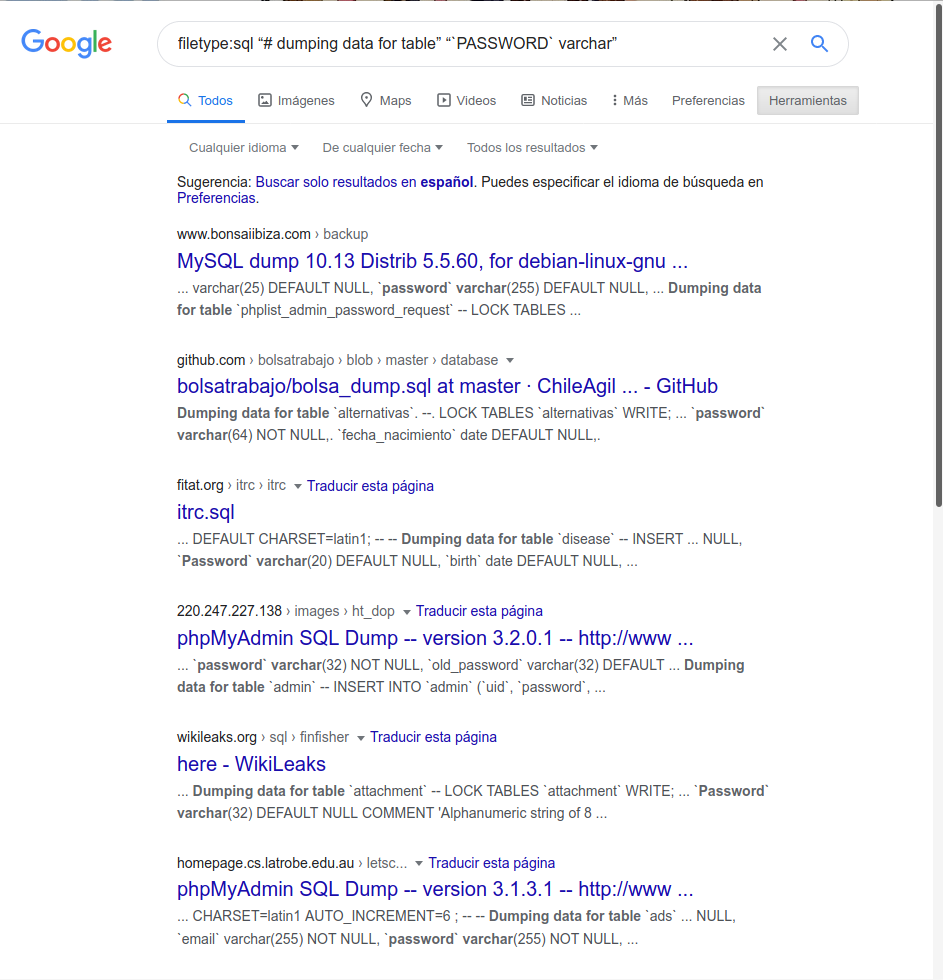
\includegraphics[width=.20\textwidth]{images/command1/base.png}\\
	
\includegraphics[width=.20\textwidth]{images/command1/result1.png}\\
	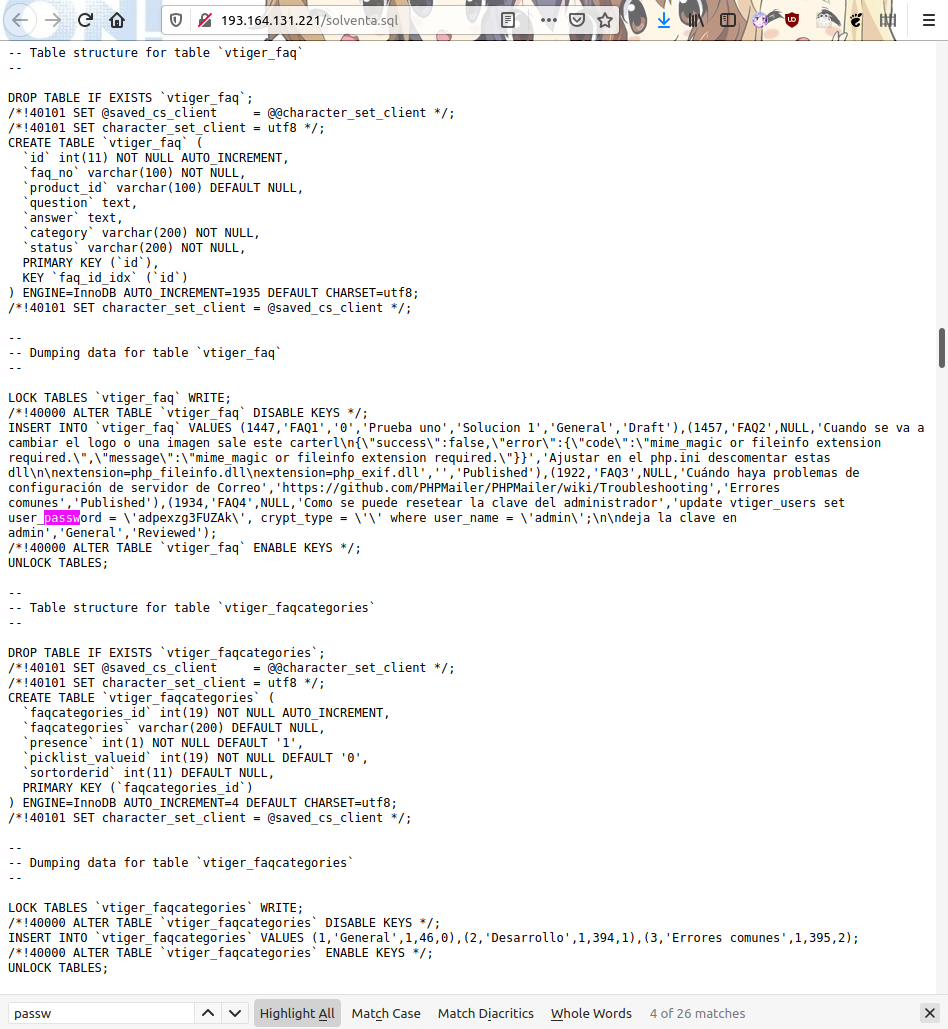
\includegraphics[width=.20\textwidth]{images/command1/result2.png}\\
	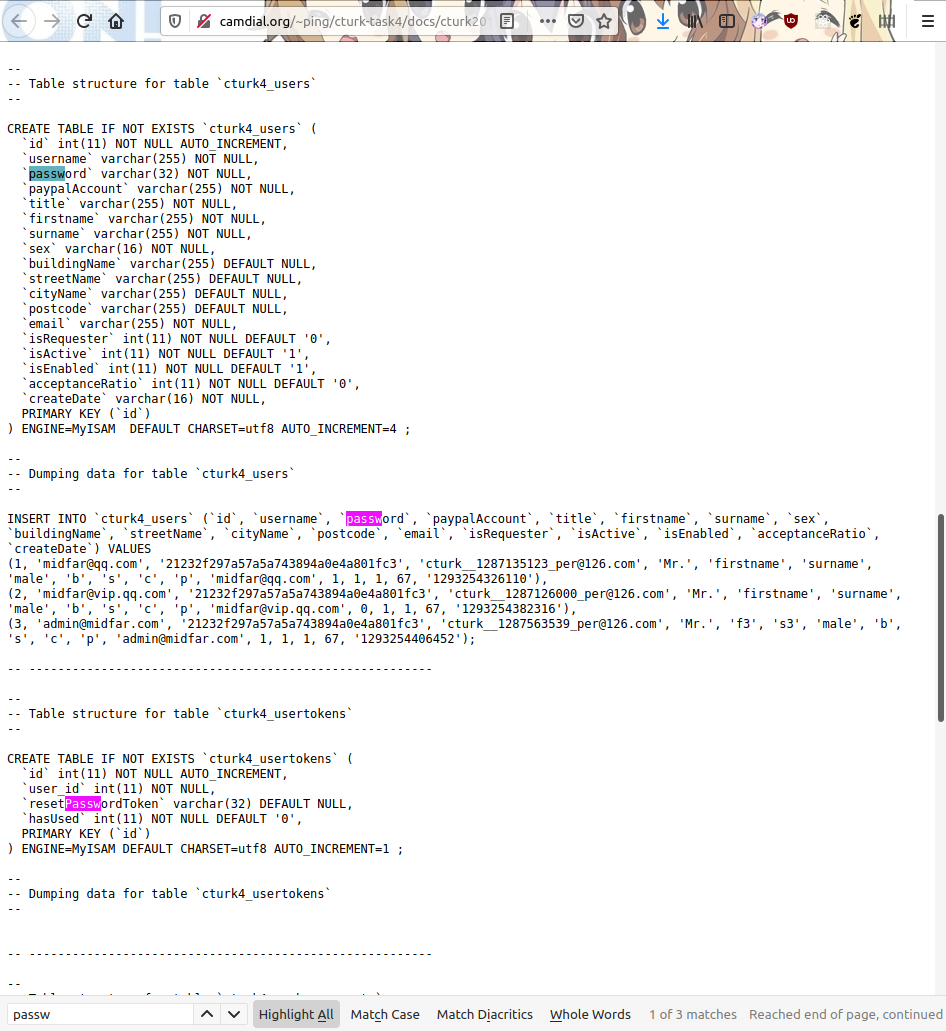
\includegraphics[width=.20\textwidth]{images/command1/result3.png}\\
\end{multicols}
\caption{Archivos de tipo sql, los cuales tengan dentro del texto \texttt{\# dumping data for table} y \texttt{`PASSWORD` varchar}, típicos de los dumps. Intenta buscar dumps con contraseñas por si alguno la volcó y dejó disponible.}
\label{FIG:command1}
\end{figure}

\subsubsection{\texttt{text:pwd inurl:(service | authors | administrators | users) \enquote*{\# -FrontPage-}\  }}
\begin{figure}[H]
	\centering
\begin{multicols}{4}
	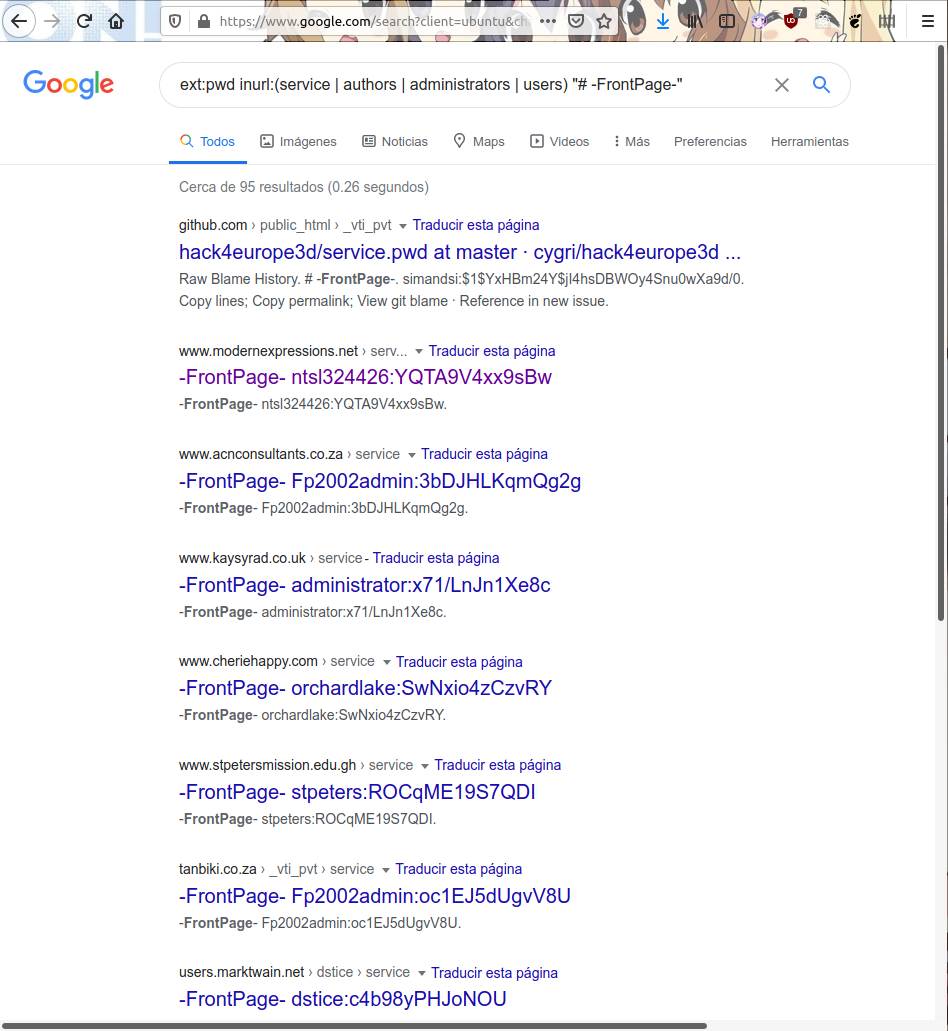
\includegraphics[width=.20\textwidth]{images/command2/base.png}\\
	
\includegraphics[width=.20\textwidth]{images/command2/result1.png}\\
	
\includegraphics[width=.20\textwidth]{images/command2/result2.png}\\
	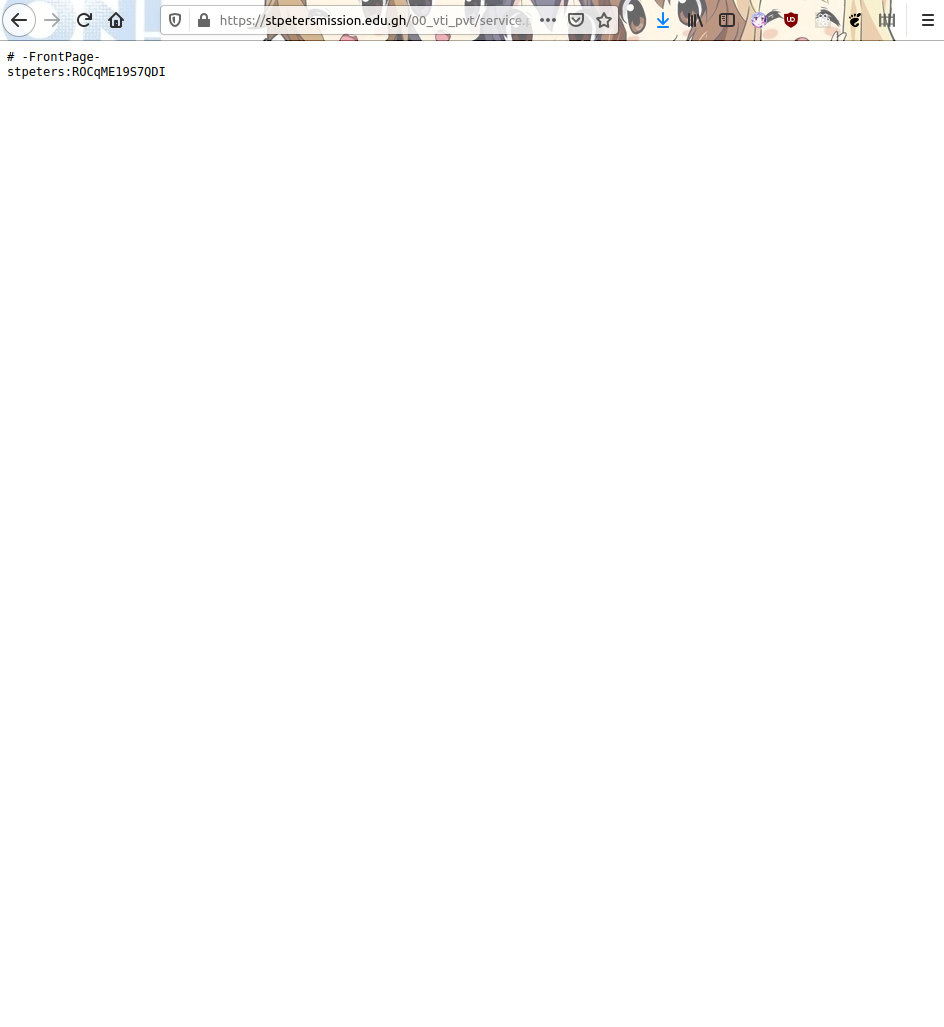
\includegraphics[width=.20\textwidth]{images/command2/result3.png}\\
\end{multicols}
\caption{Sitios con el texto \textit{pwd} que presenten match en la url \textit{(service|authors|administrators|users)} y que poseean \textit{-FrontPage-} en su resultado. Sirve para encontrar accesos en desarrollos hechos con FrontPage o Dreamweaver.}
\label{FIG:command2}
\end{figure}


\subsubsection{\texttt{inurl:/admin/login.asp}}
\begin{figure}[H]
	\centering
\begin{multicols}{4}
	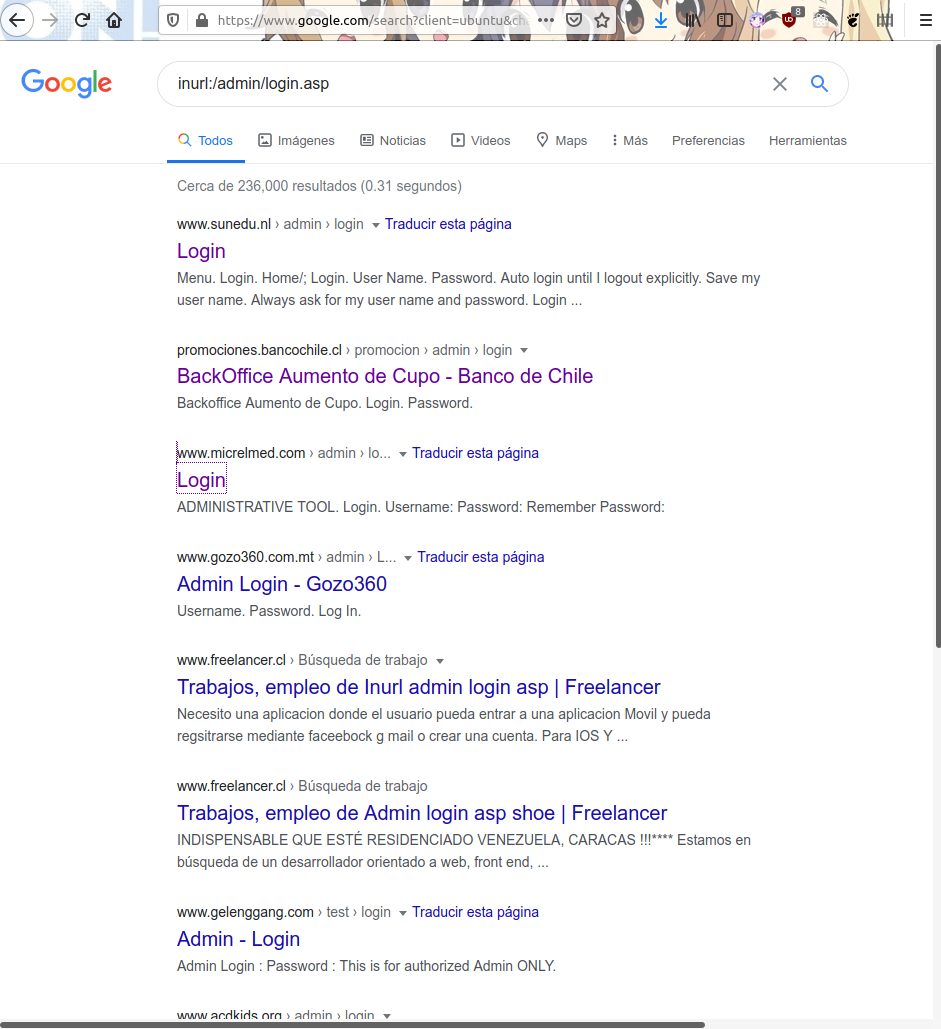
\includegraphics[width=.20\textwidth]{images/command3/base.png}\\
	
\includegraphics[width=.20\textwidth]{images/command3/result1.png}\\
	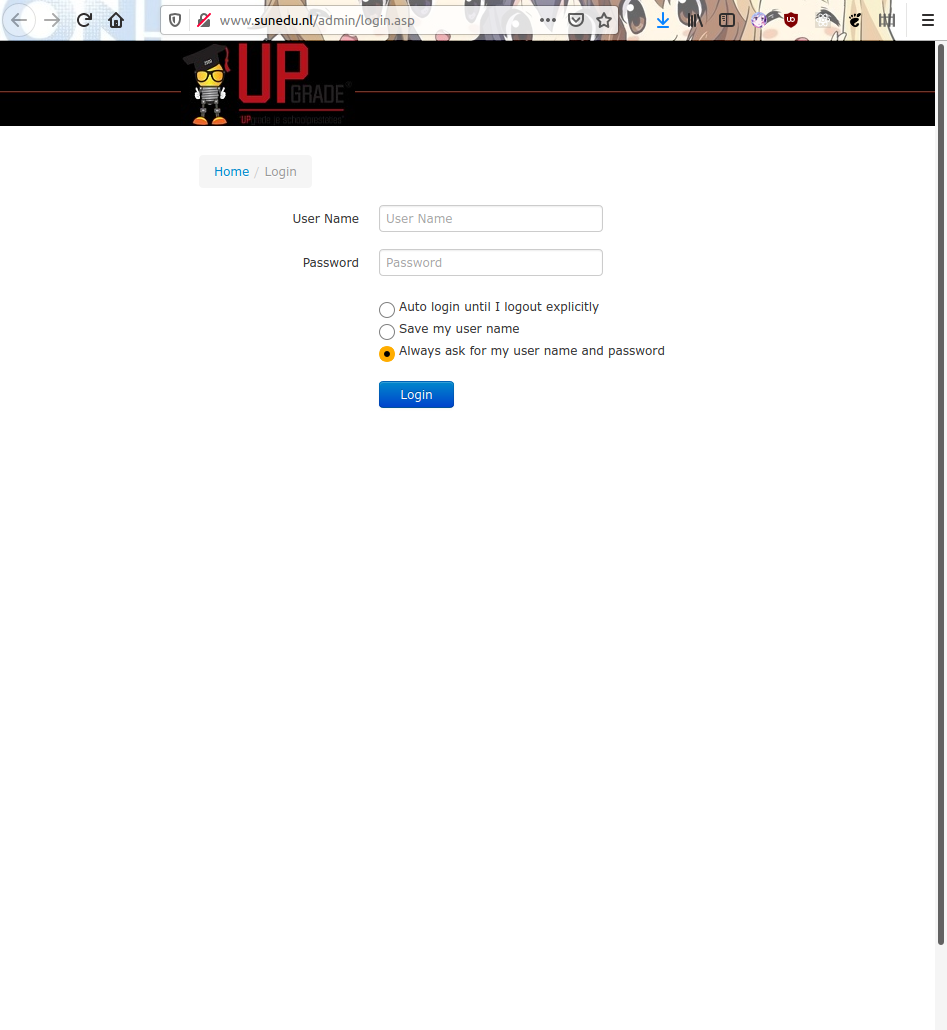
\includegraphics[width=.20\textwidth]{images/command3/result2.png}\\
	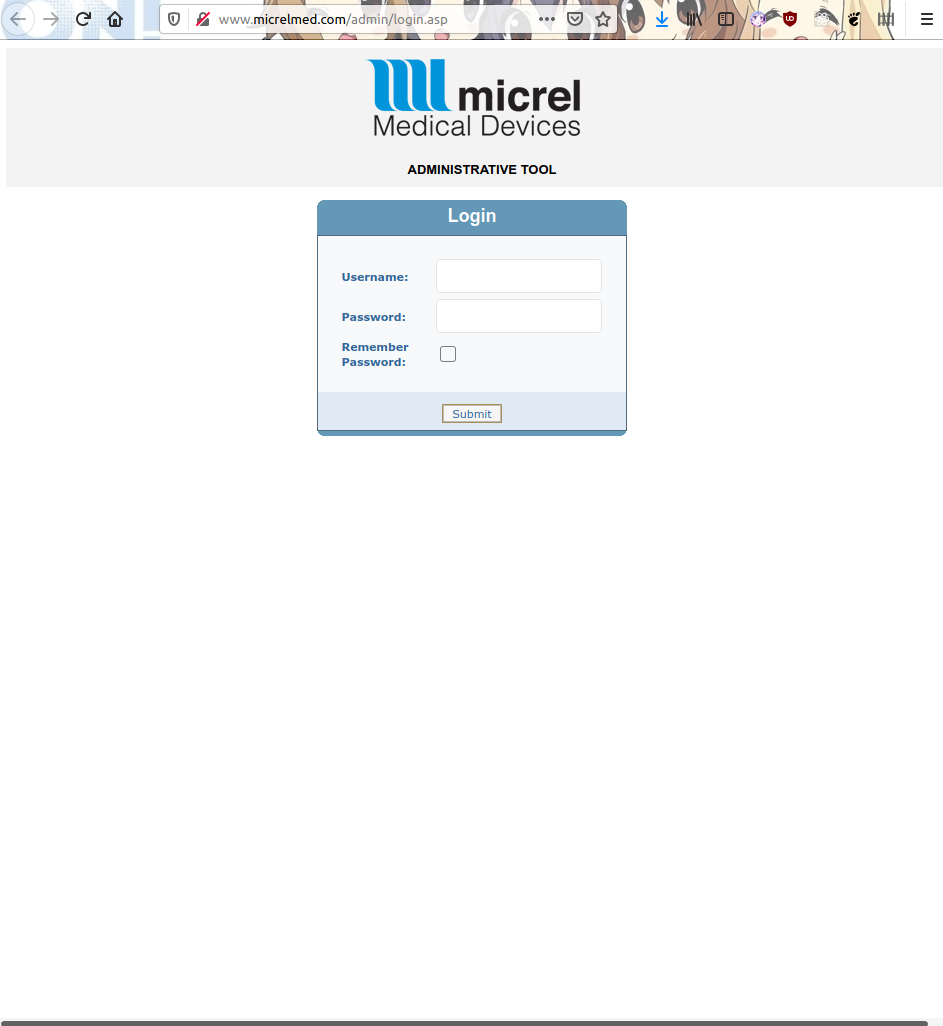
\includegraphics[width=.20\textwidth]{images/command3/result3.png}\\
\end{multicols}
\caption{URLs que encajen con \textit{/admin/login.asp}. Esas url suelen ser dejadas por desarrollos en ASP y rara vez cuentan con algun mecanismo de protección contra ataques de fuerza bruta, volviéndolas un buen objetivo para este tipo de ataques.}
\label{FIG:command3}
\end{figure}


\subsubsection{\texttt{allintitle:\enquote*{Outlook Web Access Logon}}}
\begin{figure}[H]
	\centering
\begin{multicols}{4}
	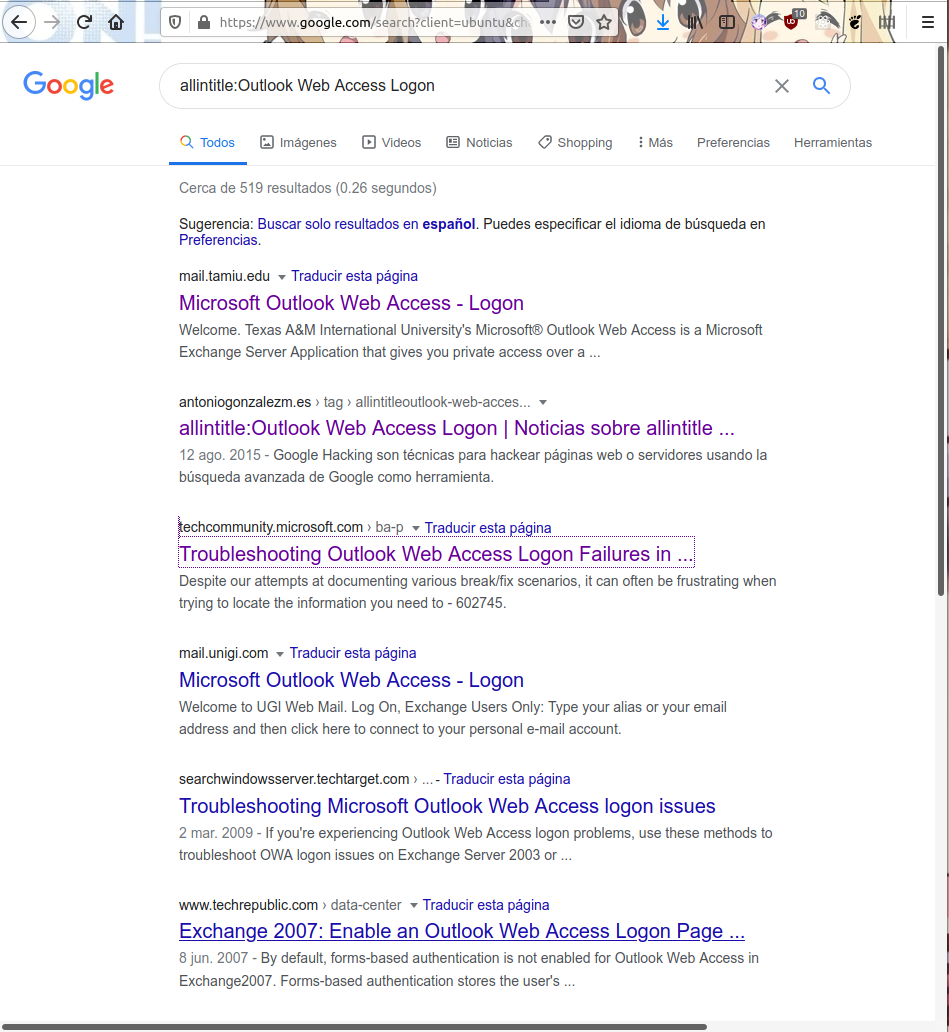
\includegraphics[width=.20\textwidth]{images/command4/base.png}\\
	
\includegraphics[width=.20\textwidth]{images/command4/result1.png}\\
	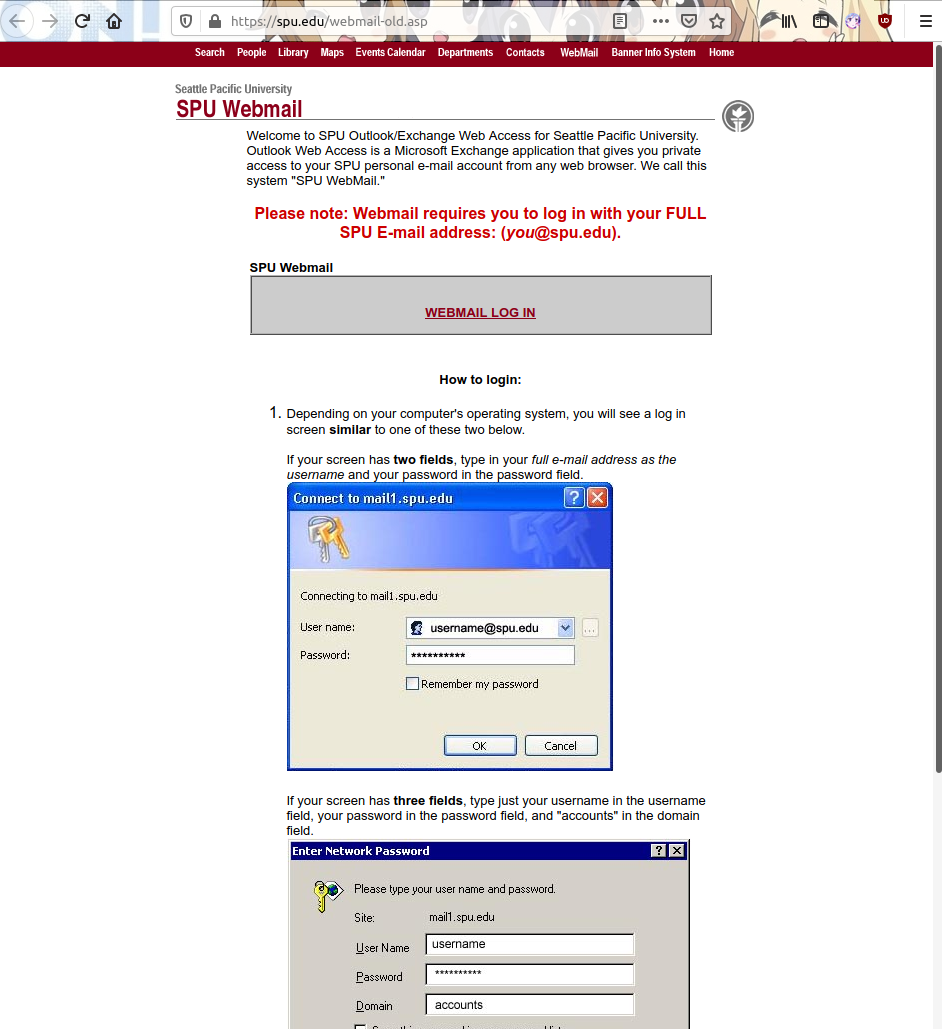
\includegraphics[width=.20\textwidth]{images/command4/result2.png}\\
	
\includegraphics[width=.20\textwidth]{images/command4/result3.png}\\
\end{multicols}
\caption{Sitios que tengan \textit{Outlook Web Access Logon} en su título.Antiguamente utilizado para encontrar puntos de acceso para servidores Outlook, pero google restringe su uso como también hay cada vez menos servidores utilizando este servicio. Un ejemplo de un comando que ha envejecido mal en el tiempo.}
\label{FIG:command4}
\end{figure}

\subsubsection{\texttt{intitle:index.of \enquote*{Apache/*} \enquote*{server at}}}
\begin{figure}[H]
	\centering
\begin{multicols}{4}
	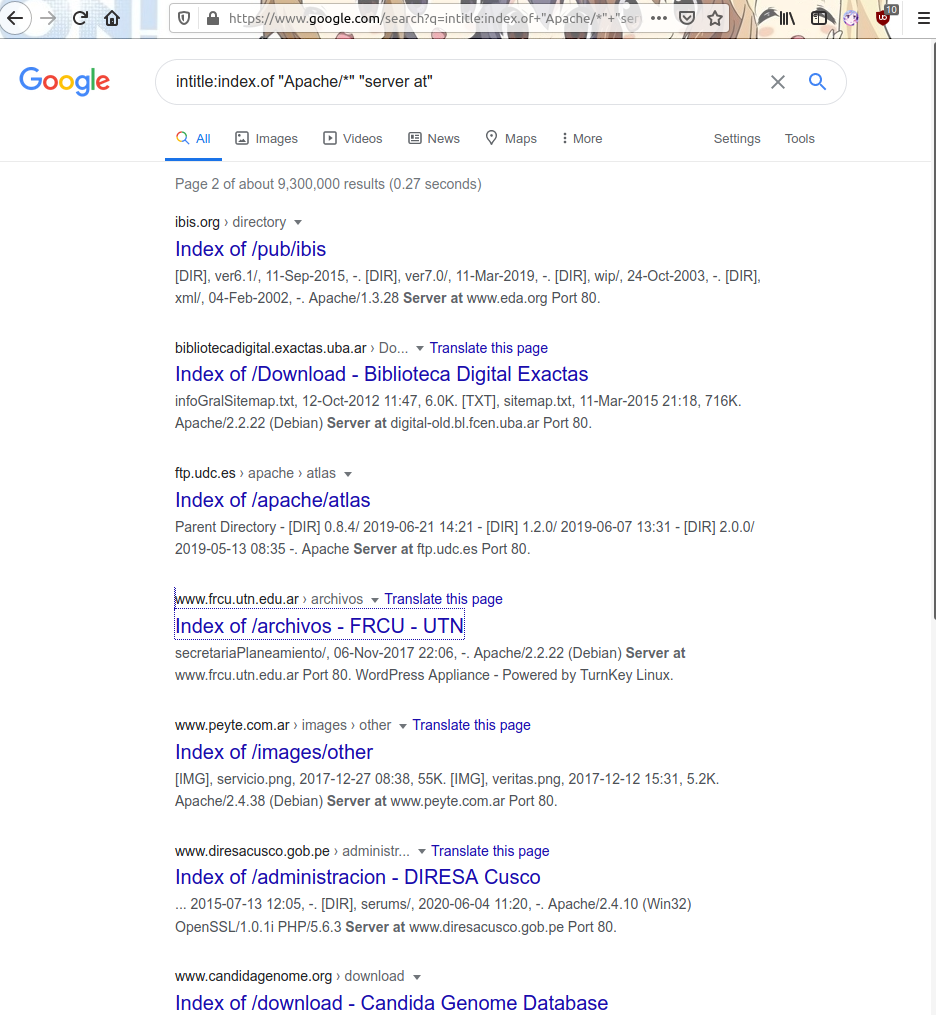
\includegraphics[width=.20\textwidth]{images/command5/base.png}\\
	
\includegraphics[width=.20\textwidth]{images/command5/result1.png}\\
	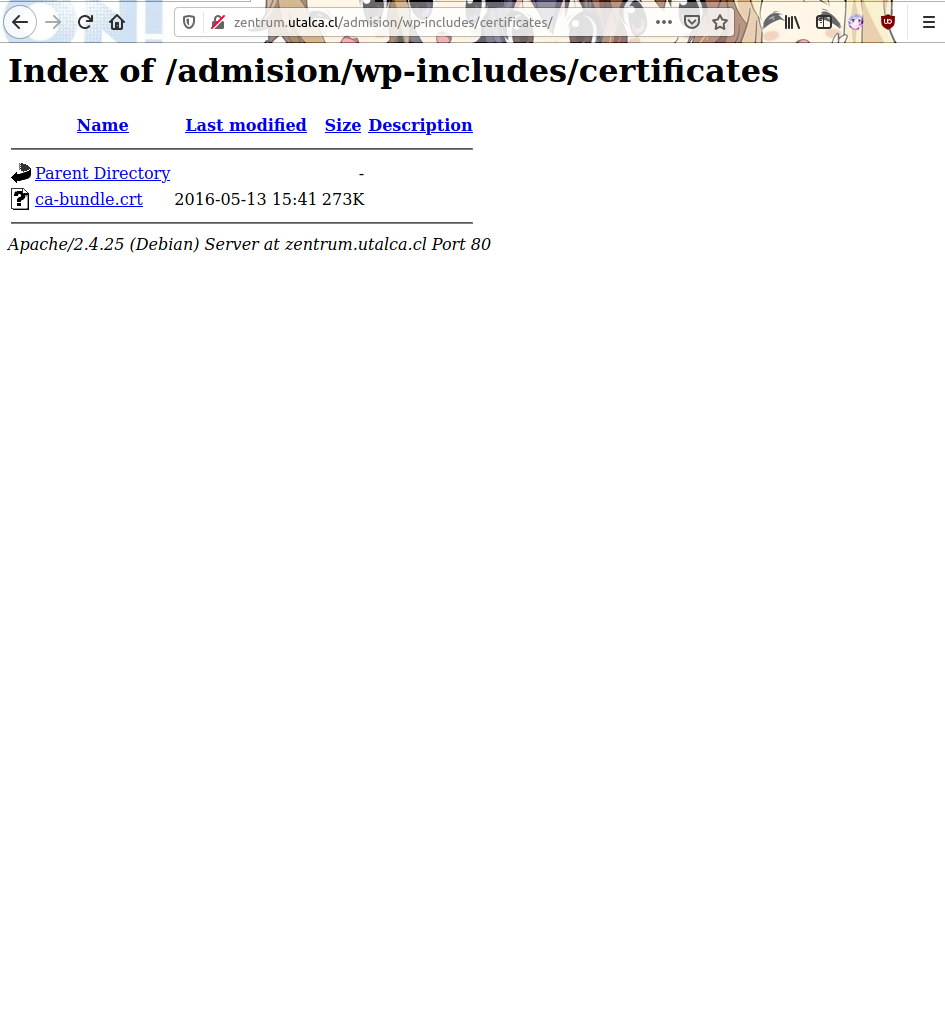
\includegraphics[width=.20\textwidth]{images/command5/result2.png}\\
	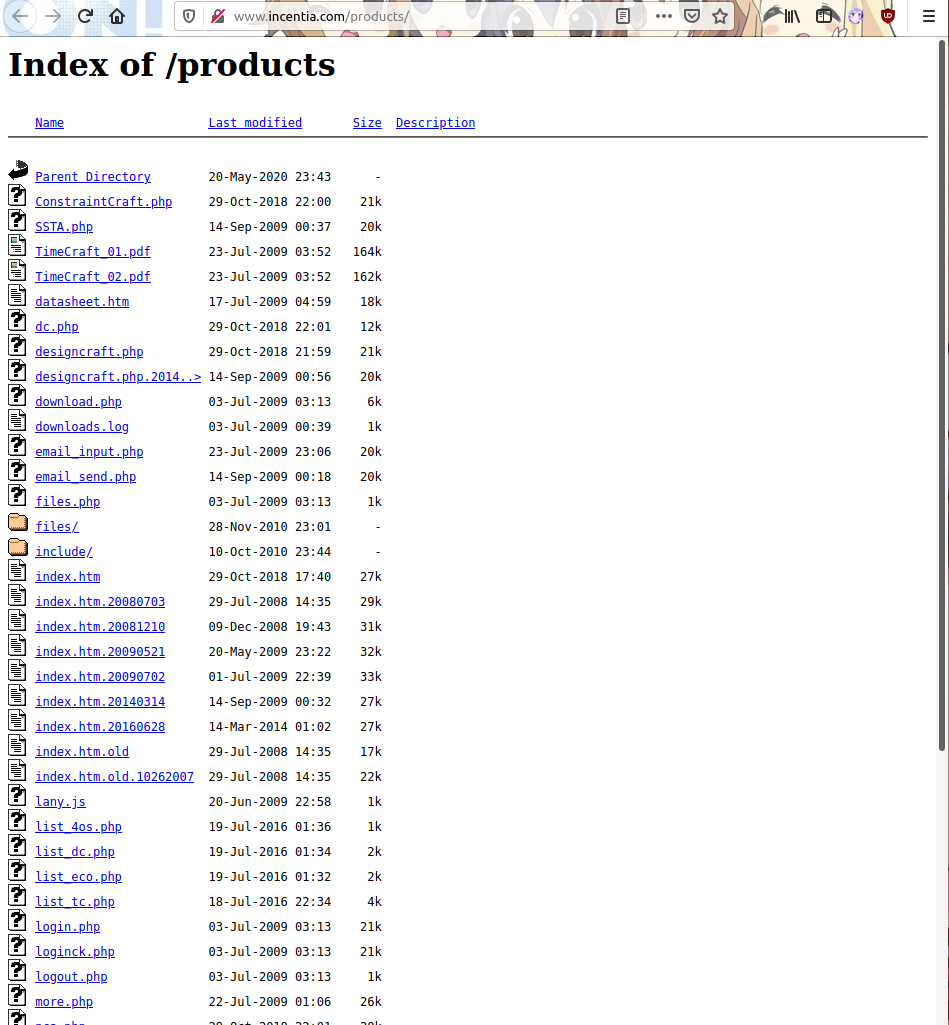
\includegraphics[width=.20\textwidth]{images/command5/result3.png}\\
\end{multicols}
\caption{Sitios que tengan match \textit{(index.of)?(.*)(Apache/*)(.*)(server at)} en su título. Ese título es el titulo que tiene por defecto el webroot en los servidores Apache, que muchos olvidan desactivar. El hecho que esté activo da la oportunidad de explorar el sistema de archivos local que está montado en el mismo lo cual puede filtrar documentos.}
\label{FIG:command5}
\end{figure}



\subsubsection{\texttt{\enquote*{SquirrelMail version 1.4.4} inurl:src ext:php}}
\begin{figure}[H]
	\centering
\begin{multicols}{4}
	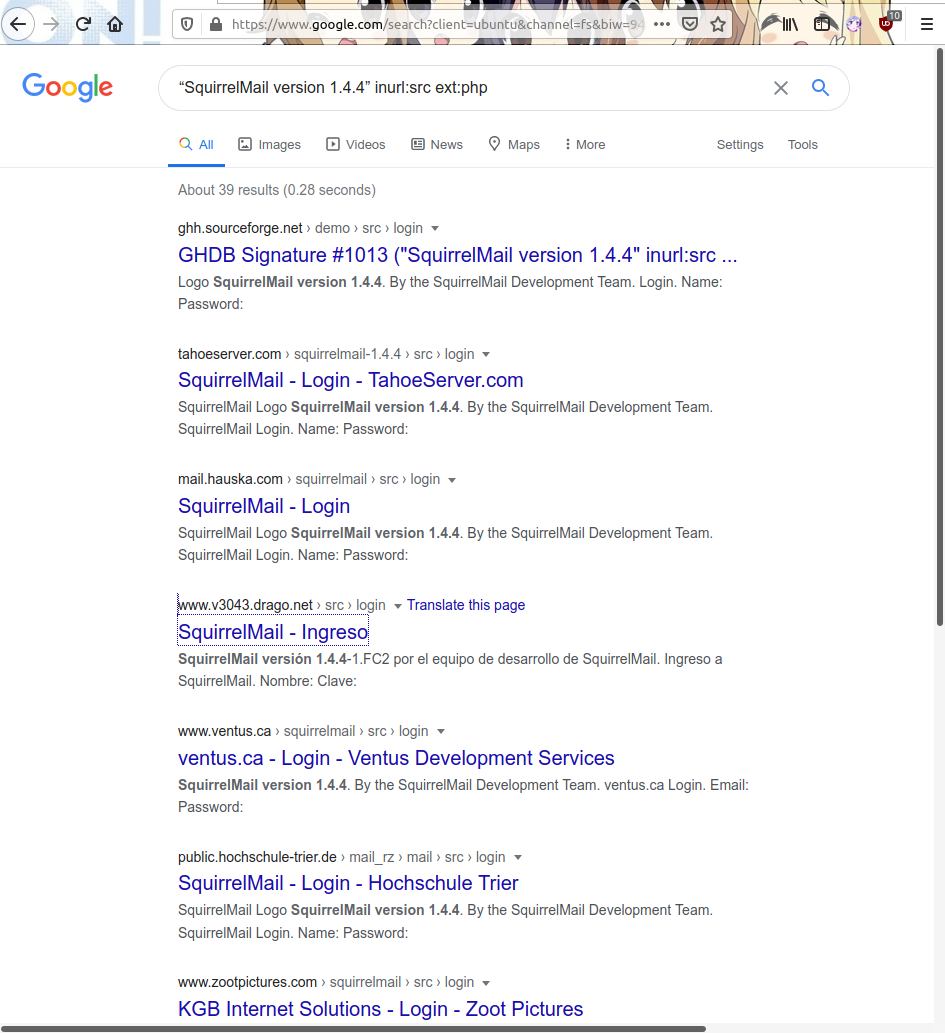
\includegraphics[width=.20\textwidth]{images/command6/base.png}\\
	
\includegraphics[width=.20\textwidth]{images/command6/result1.png}\\
	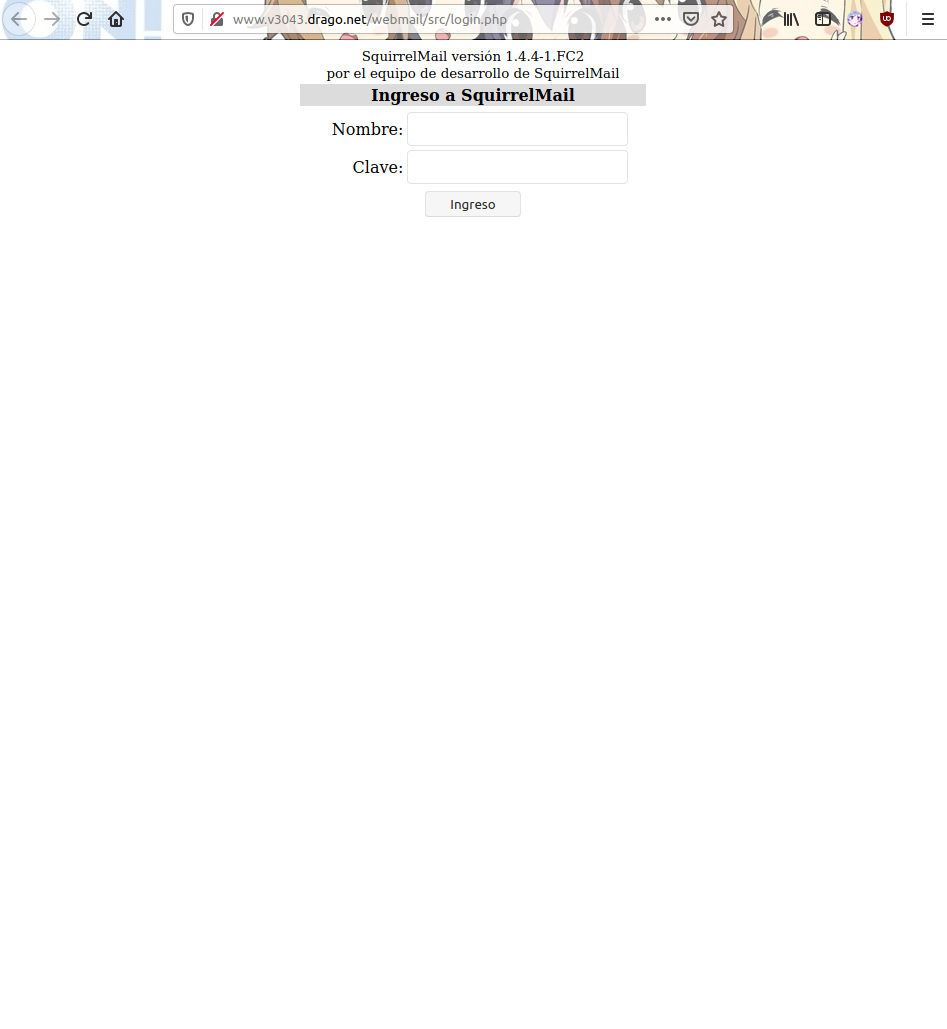
\includegraphics[width=.20\textwidth]{images/command6/result2.png}\\
	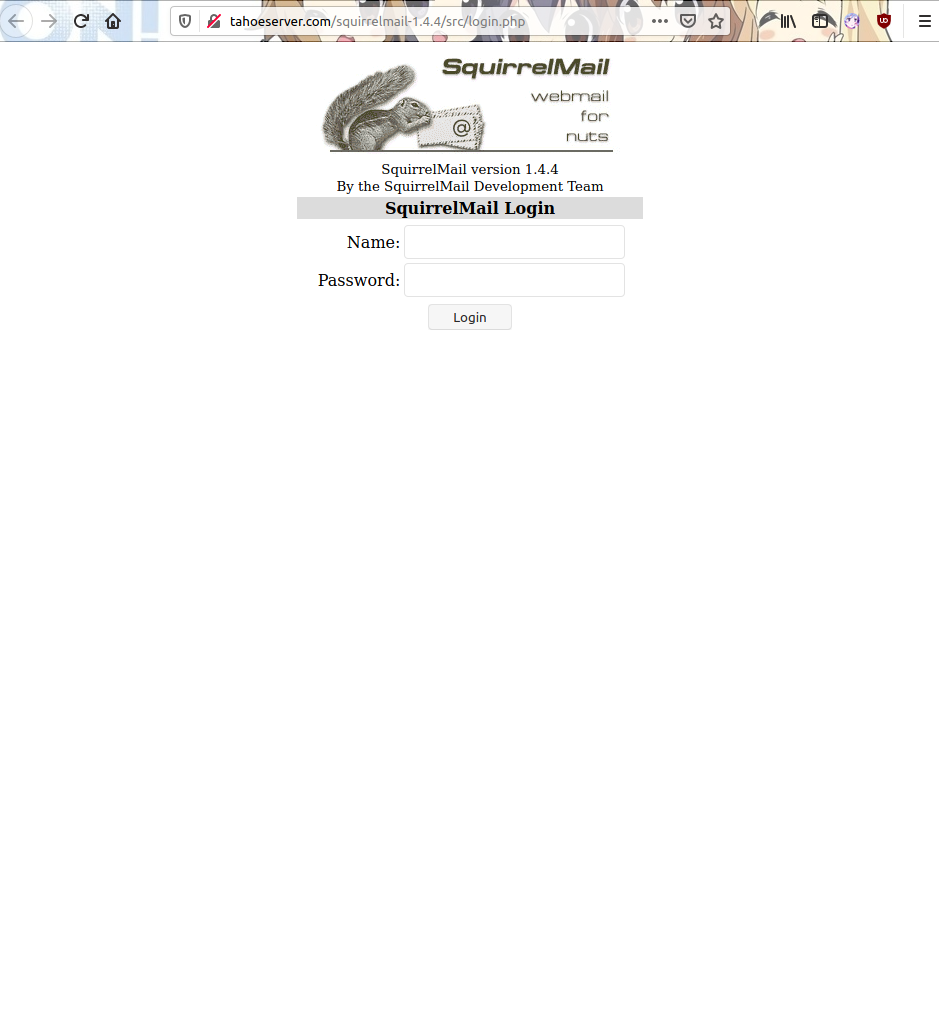
\includegraphics[width=.20\textwidth]{images/command6/result3.png}\\
\end{multicols}
\caption{Sitios que tengan match \textit{SquirrelMail version 1.4.4}. Exactamente la misma idea de buscar puntos de entrada a servidores outlook, pero esta vez con SquirrelMail.}
\label{FIG:command6}
\end{figure}


\subsubsection{\texttt{camera linksys inurl:main.cgi}}
\begin{figure}[H]
	\centering
\begin{multicols}{4}
	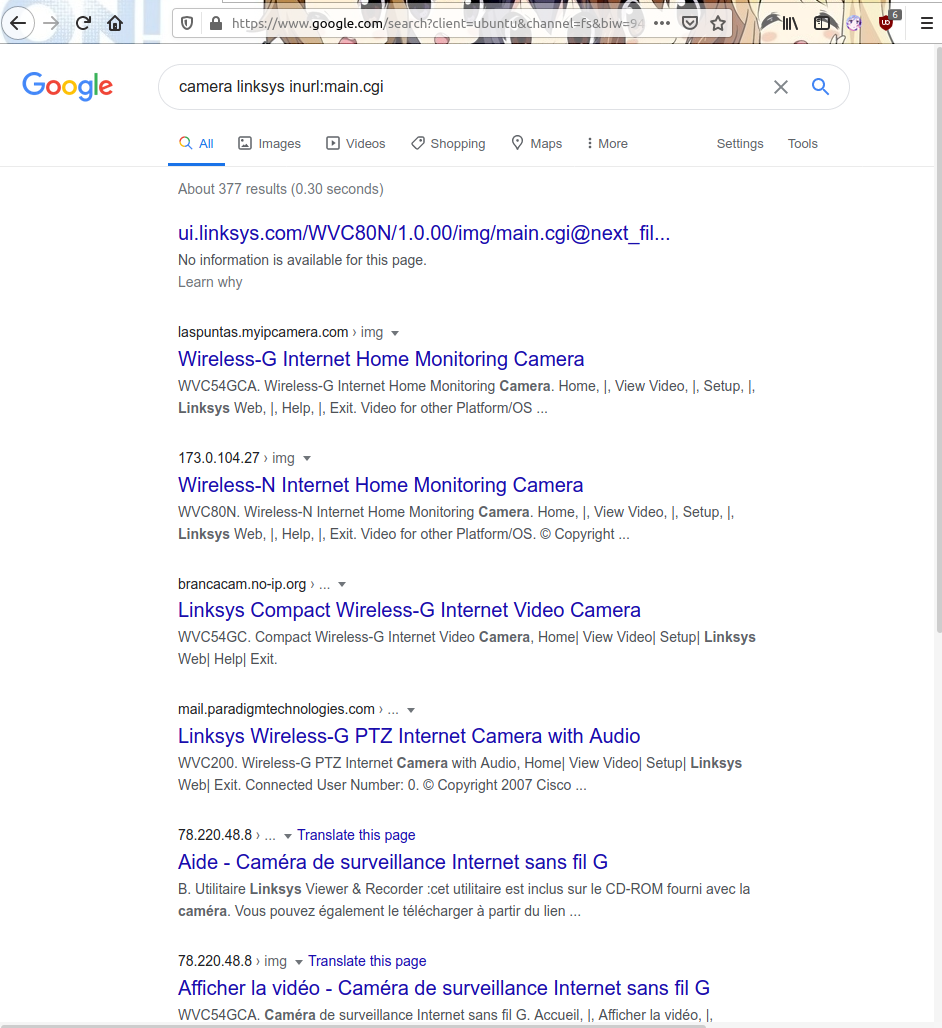
\includegraphics[width=.20\textwidth]{images/command7/base.png}\\
	
\includegraphics[width=.20\textwidth]{images/command7/result1.png}\\
	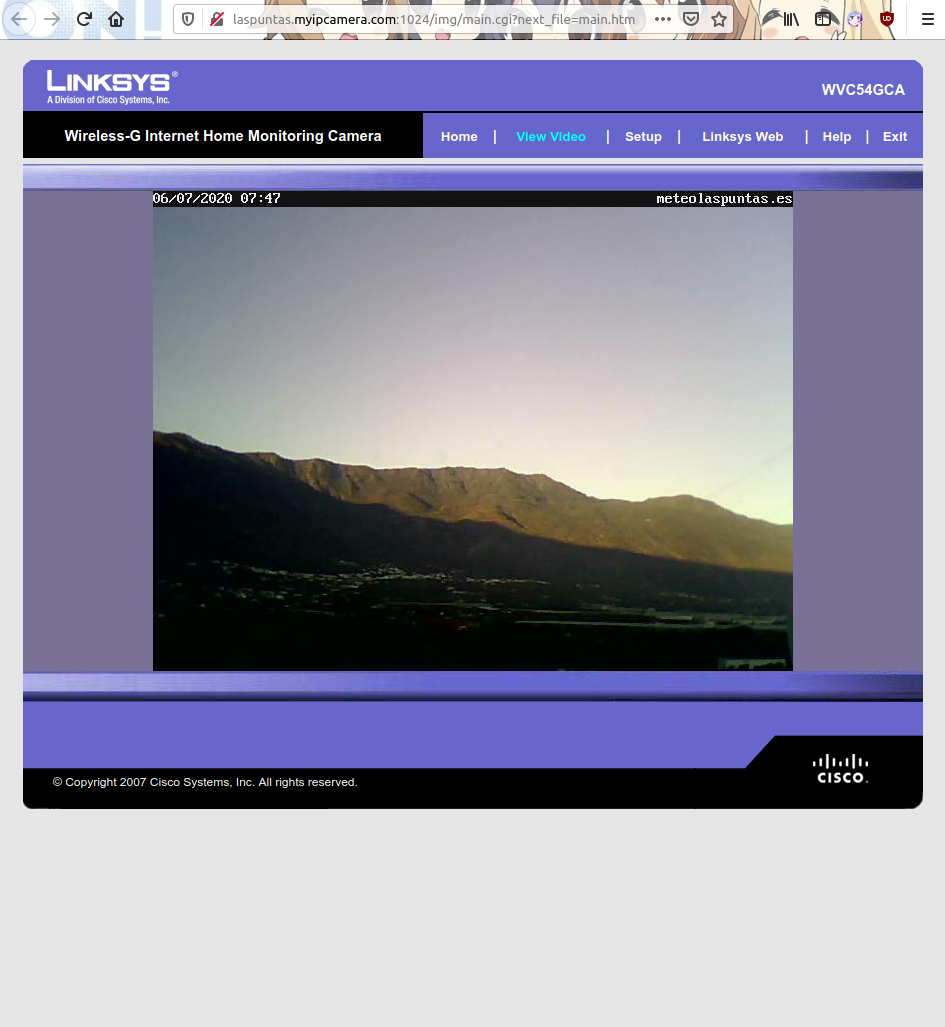
\includegraphics[width=.20\textwidth]{images/command7/result2.png}\\
	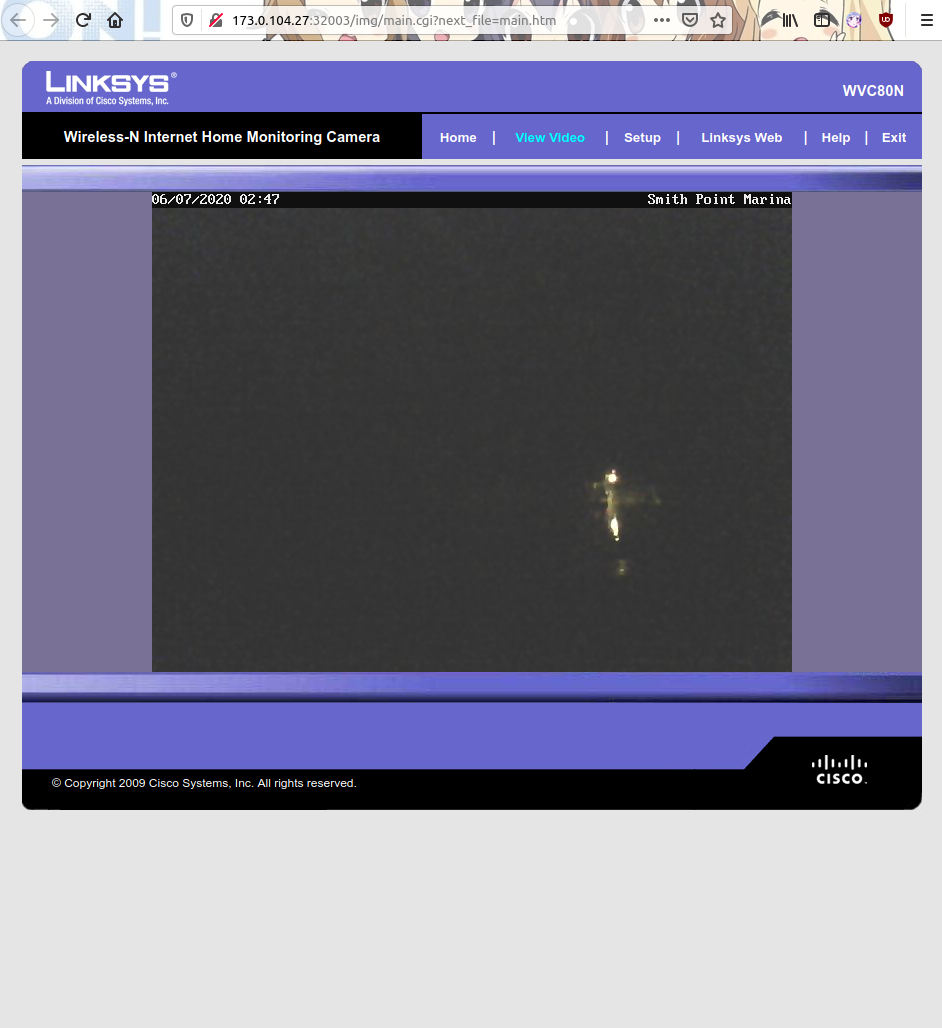
\includegraphics[width=.20\textwidth]{images/command7/result3.png}\\
\end{multicols}
\caption{Sitios que tengan match \textit{camera linksys inurl:main.cgi}. Muchas cámaras lynksys son configuradas para acceder a internet directamente en modo puente y a la gente se les olvida ponerles protección, permitiendo ver lo que transmiten.}
\label{FIG:command7}
\end{figure}



\subsubsection{\texttt{inurl:\enquote*{ViewerFrame?Mode=}}}
\begin{figure}[H]
	\centering
\begin{multicols}{4}
	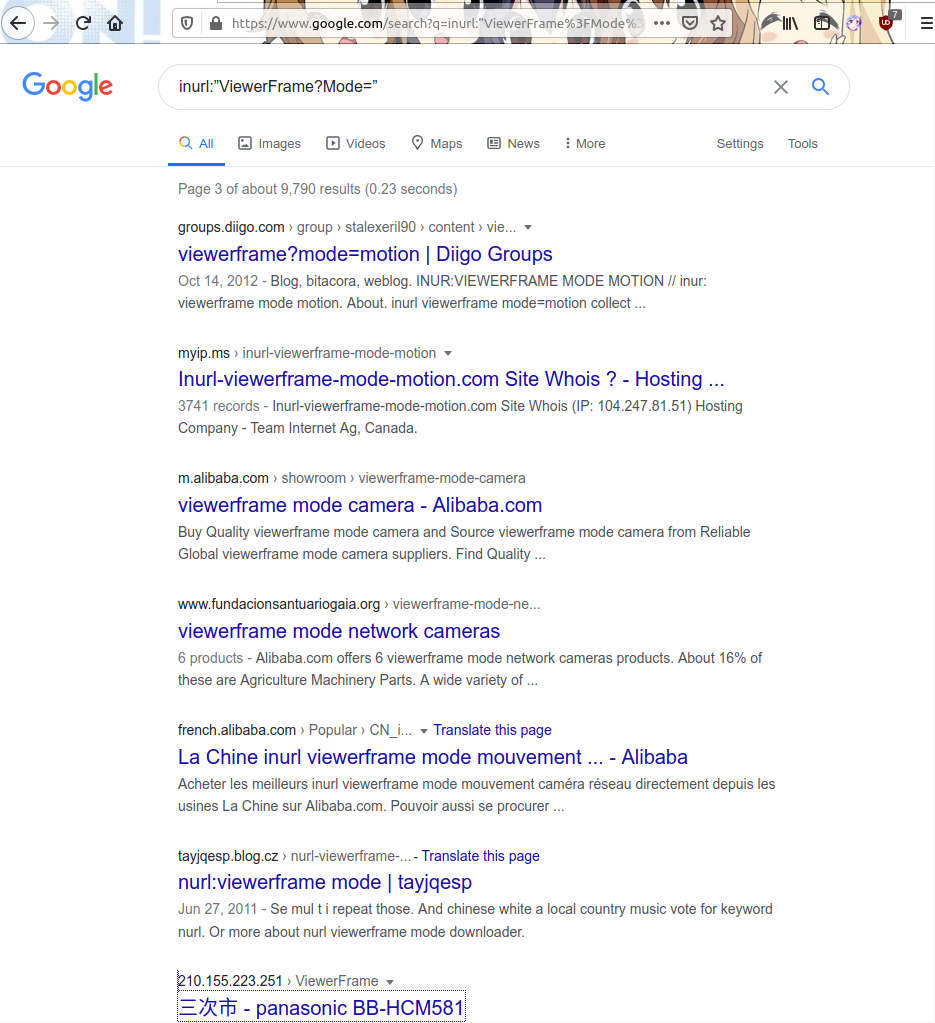
\includegraphics[width=.20\textwidth]{images/command8/base.png}\\
	
\includegraphics[width=.20\textwidth]{images/command8/result1.png}\\
	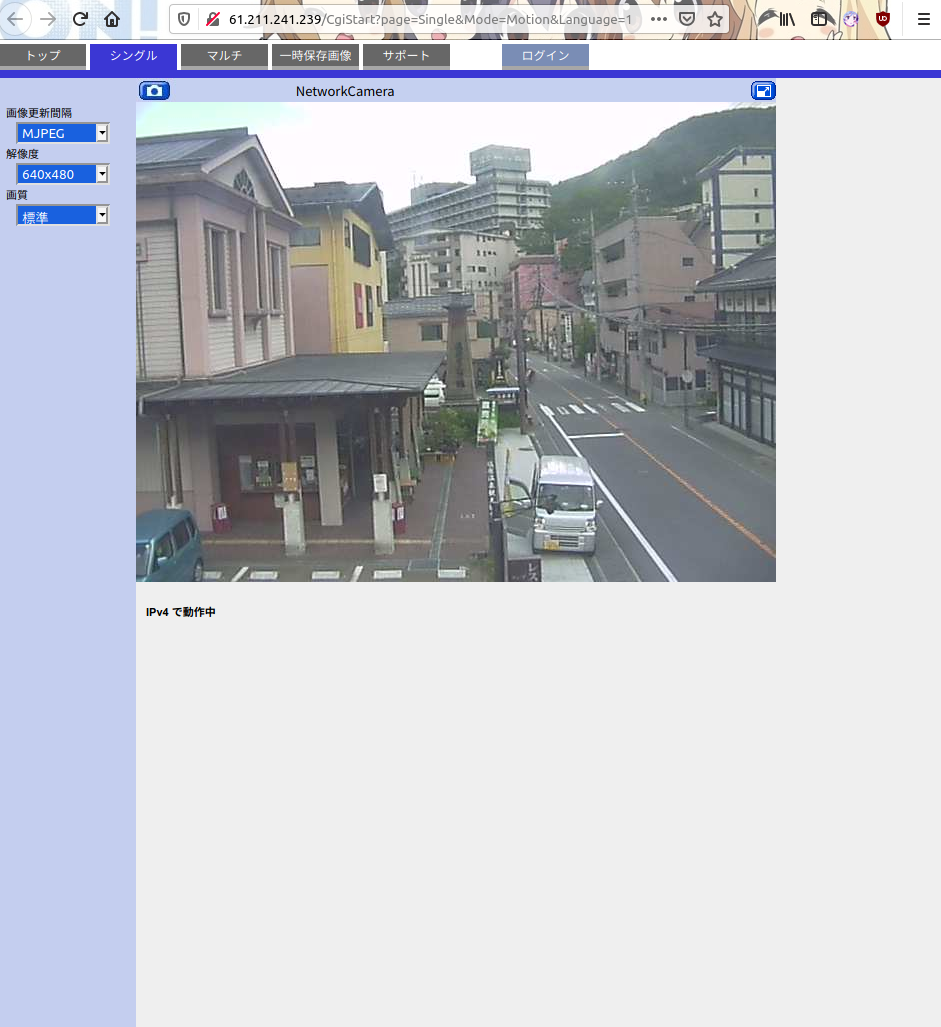
\includegraphics[width=.20\textwidth]{images/command8/result2.png}\\
	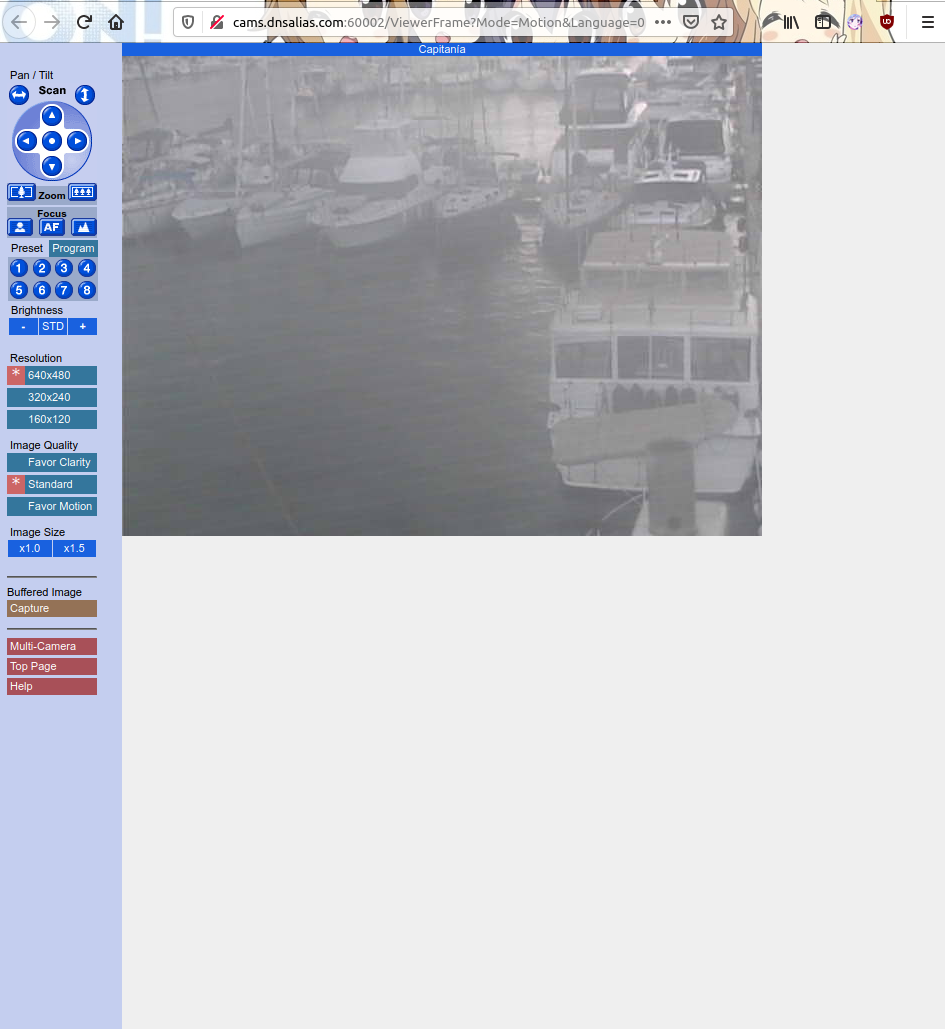
\includegraphics[width=.20\textwidth]{images/command8/result3.png}\\
\end{multicols}
\caption{Sitios que tengan match \textit{\enquote*{ViewerFrame?Mode=}} en su URL. Misma idea de las camaras lynksys anterior pero en este caso apuntando a un tipo de interfaz en específico.}
\label{FIG:command8}
\end{figure}


\subsubsection{\texttt{inurl:\enquote*{inurl:webarch/mainframe.cgi}}}
\begin{figure}[H]
	\centering
\begin{multicols}{4}
	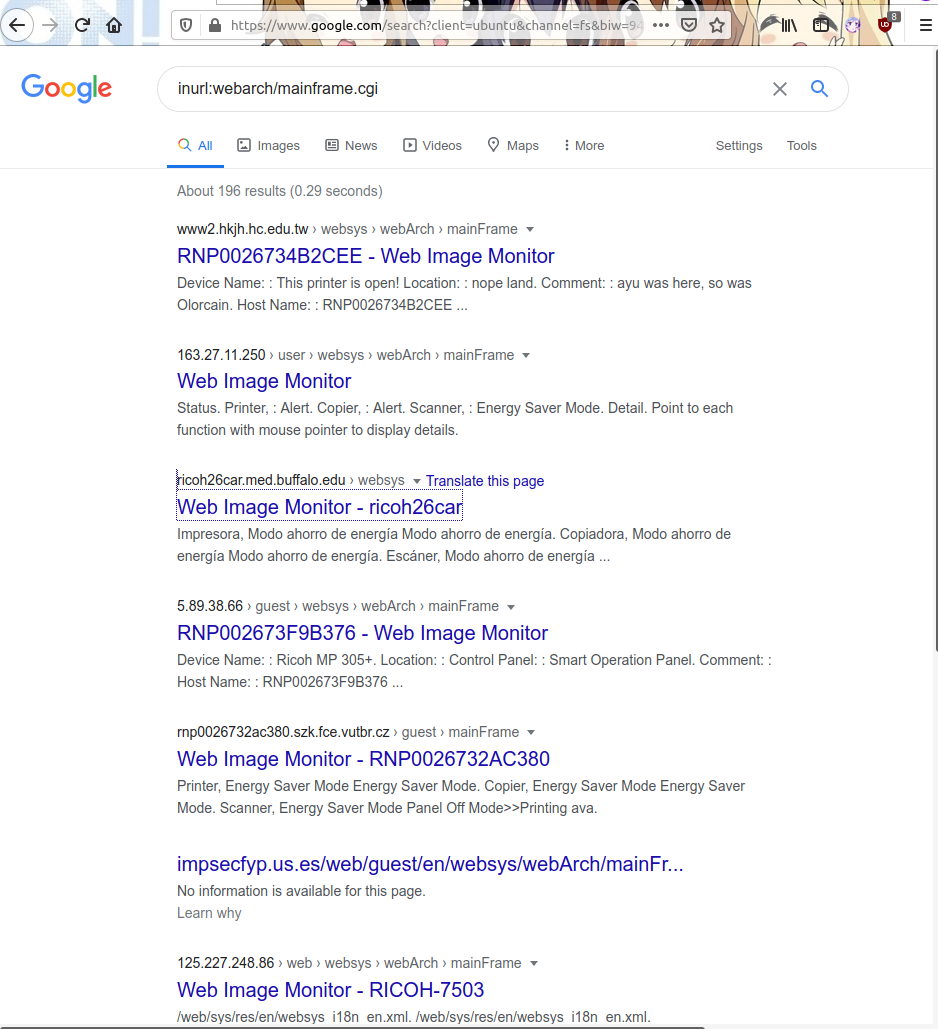
\includegraphics[width=.20\textwidth]{images/command9/base.png}\\
	
\includegraphics[width=.20\textwidth]{images/command9/result1.png}\\
	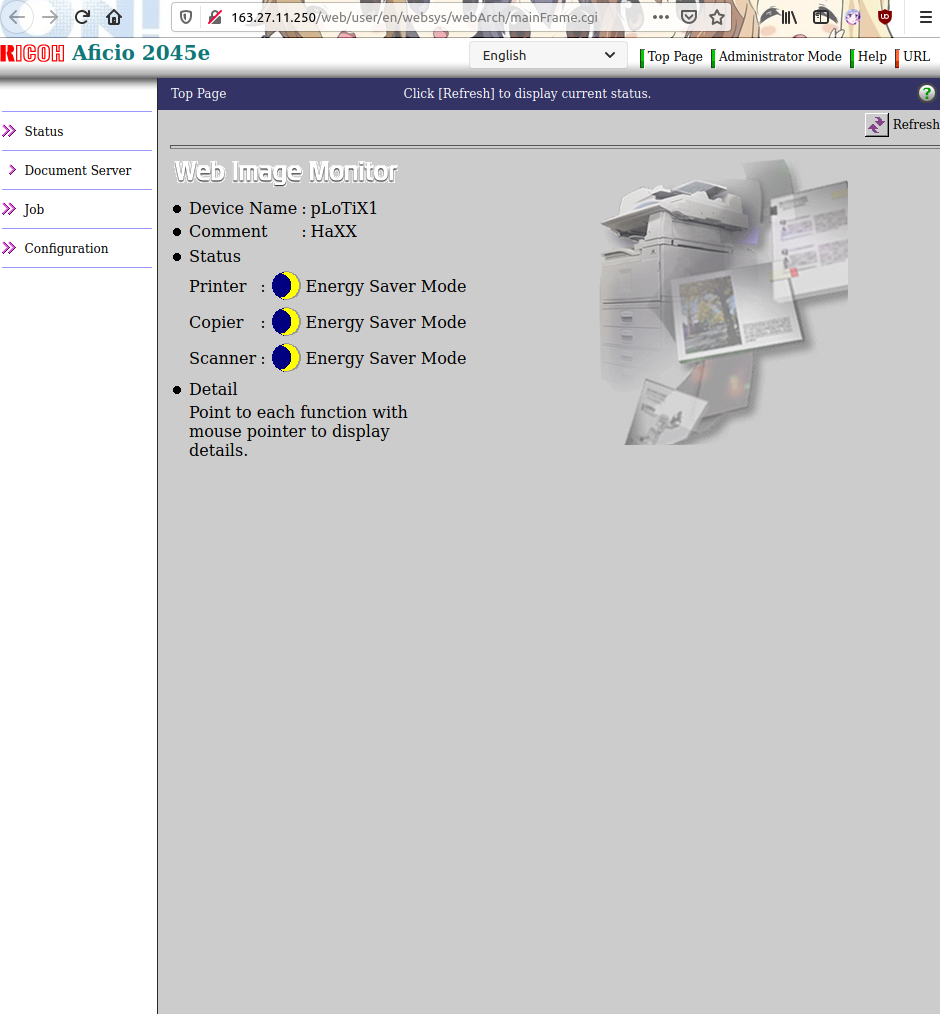
\includegraphics[width=.20\textwidth]{images/command9/result2.png}\\
	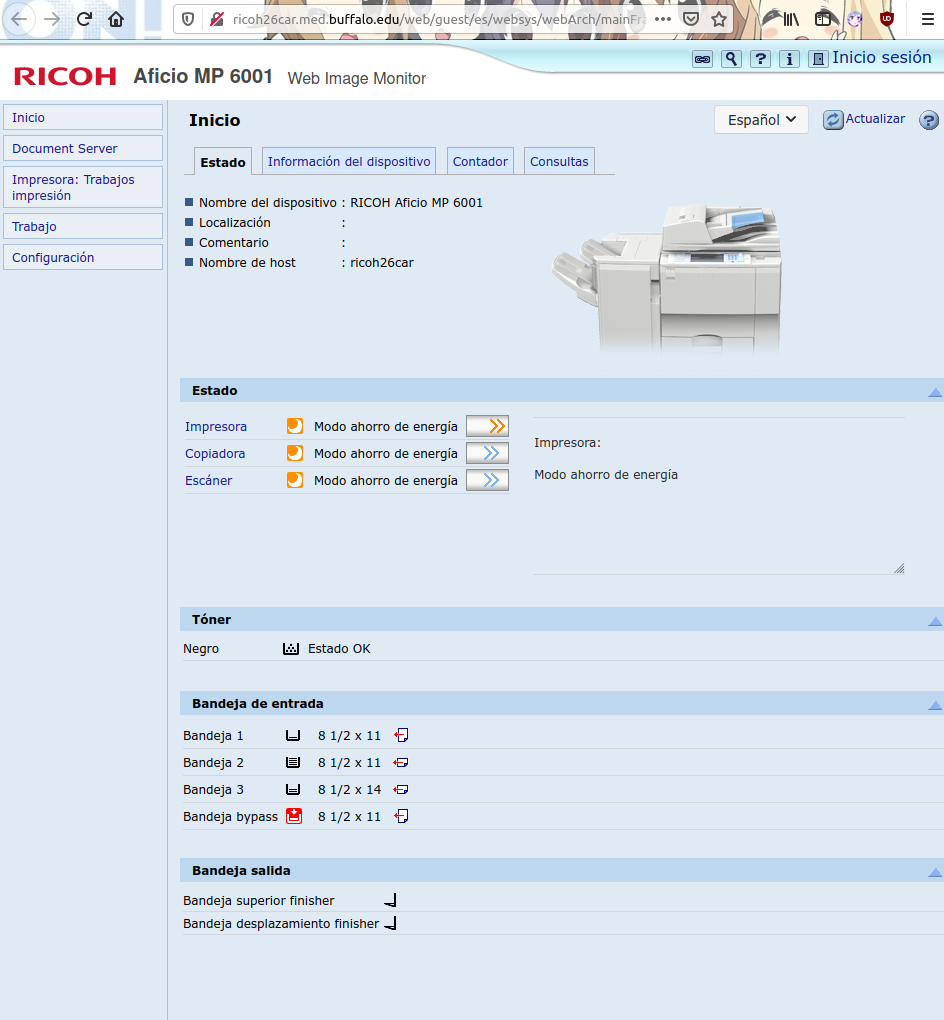
\includegraphics[width=.20\textwidth]{images/command9/result3.png}\\
\end{multicols}
\caption{Sitios que tengan match \textit{\enquote*{inurl:webarch/mainframe.cgi}} en su URL. En este caso apunta a impresoras de la marca Ricoh expuestas directamente a internet.}
\label{FIG:command9}
\end{figure}



\subsubsection{\texttt{intitle:\enquote*{network print server} filetype:shtm}}
\begin{figure}[H]
	\centering
\begin{multicols}{4}
	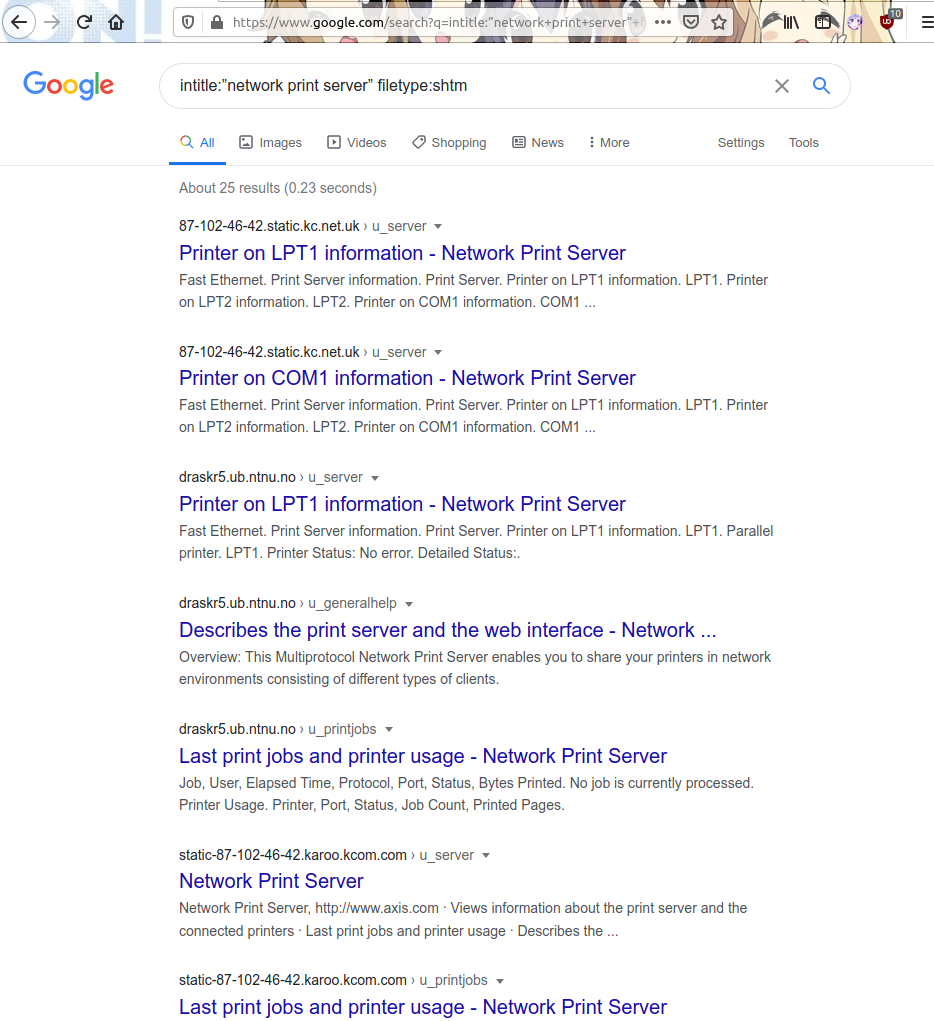
\includegraphics[width=.20\textwidth]{images/command10/base.png}\\
	
\includegraphics[width=.20\textwidth]{images/command10/result1.png}\\
	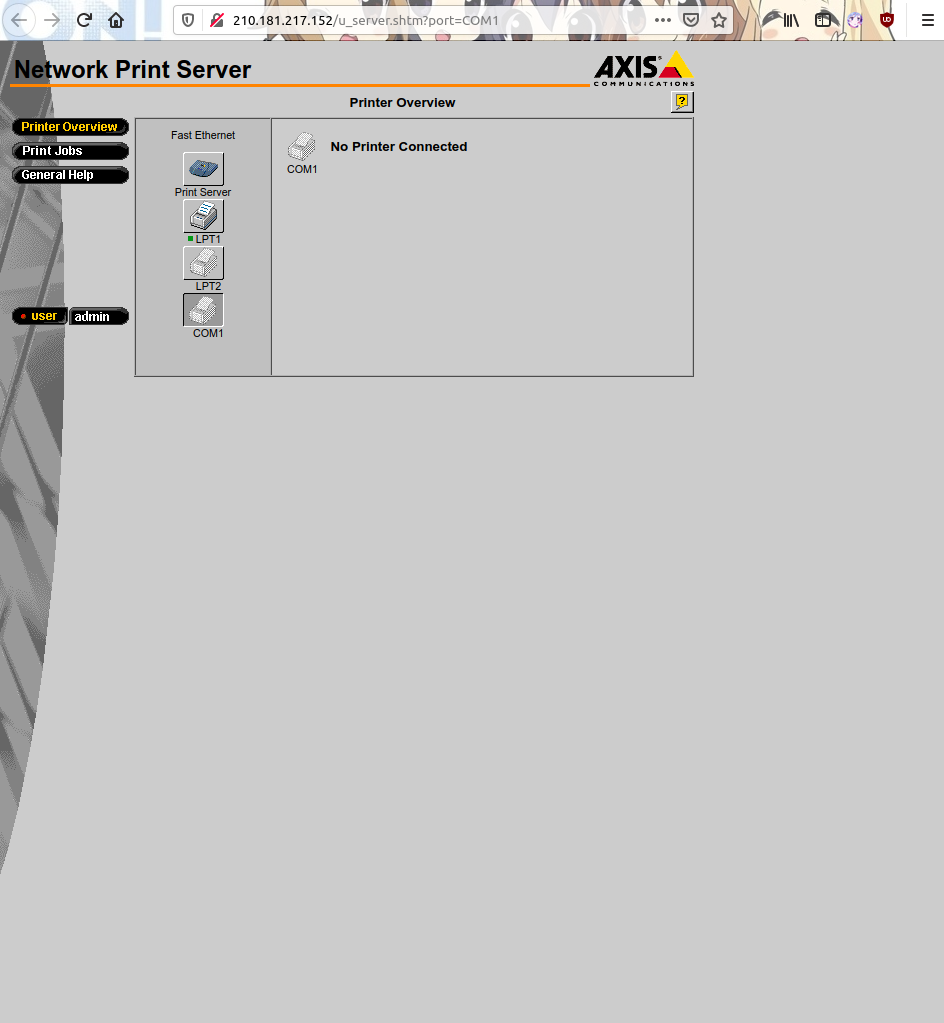
\includegraphics[width=.20\textwidth]{images/command10/result2.png}\\
	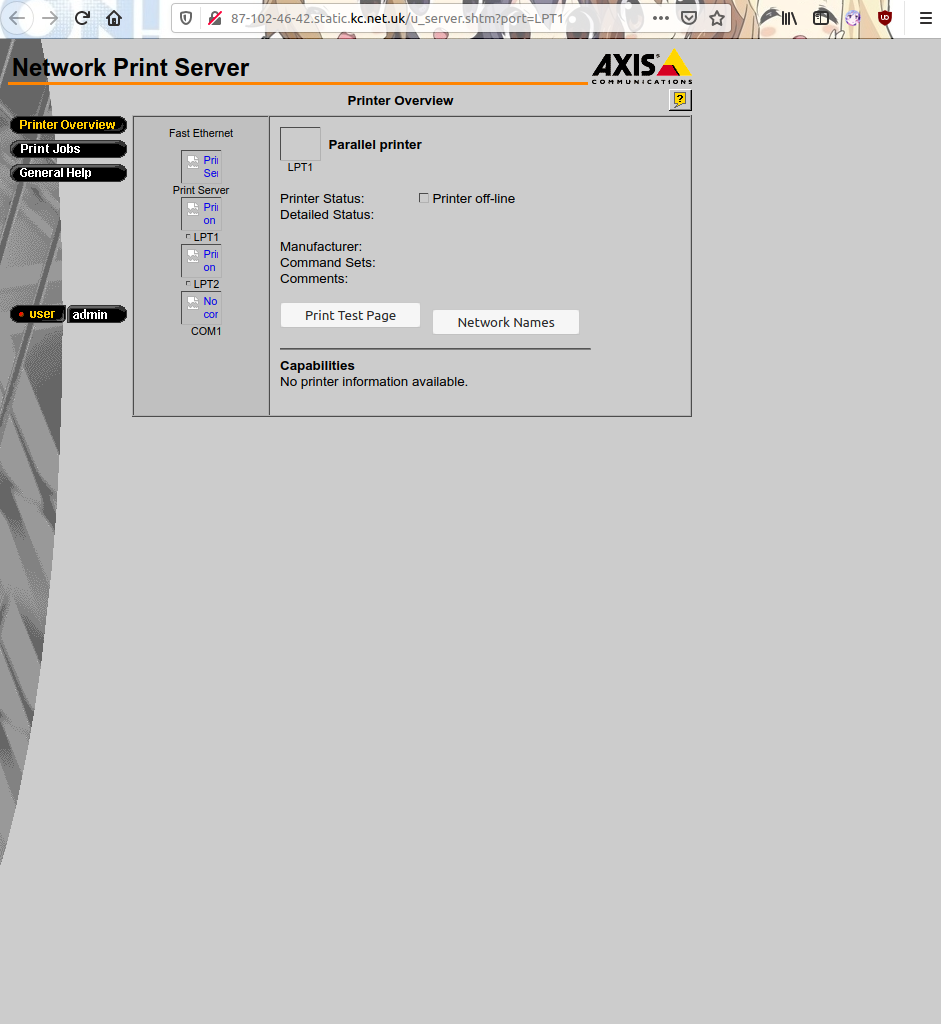
\includegraphics[width=.20\textwidth]{images/command10/result3.png}\\
\end{multicols}
\caption{Sitios que tengan match \textit{\enquote*{network print server}} en su título y que sean del tipo shtm. Busca impresoras expuestas a internet operando con el servicio de Axis Print System.}
\label{FIG:command10}
\end{figure}


\subsubsection{\texttt{ \enquote*{phone * * *} \enquote*{address *} \enquote*{e-mail} intitle: \enquote*{curriculum vitae} }}
\begin{figure}[H]
	\centering
\begin{multicols}{4}
	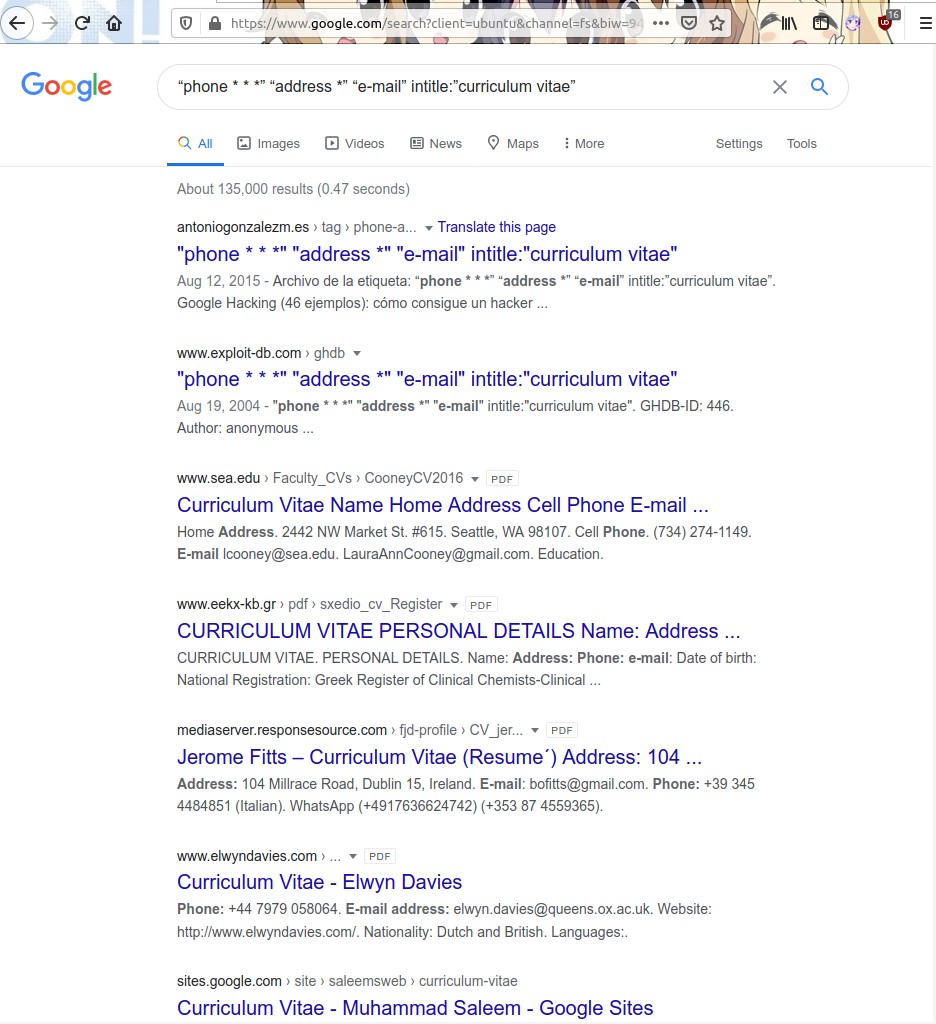
\includegraphics[width=.20\textwidth]{images/command11/base.png}\\
	
\includegraphics[width=.20\textwidth]{images/command11/result1.png}\\
	
\includegraphics[width=.20\textwidth]{images/command11/result2.png}\\
	
\includegraphics[width=.20\textwidth]{images/command11/result3.png}\\
\end{multicols}
\caption{Sitios que tengan match \textit{((phone|address|e-mail).+)*} en su contenido y que en su título indique \textit{curriculum vitae}. Busca curriculums en ingles, puede ser útil para realizar doxxing.}
\label{FIG:command11}
\end{figure}


\subsubsection{\texttt{ \enquote*{robots.txt} \enquote*{disallow:} filetype:txt}}
\begin{figure}[H]
	\centering
\begin{multicols}{4}
	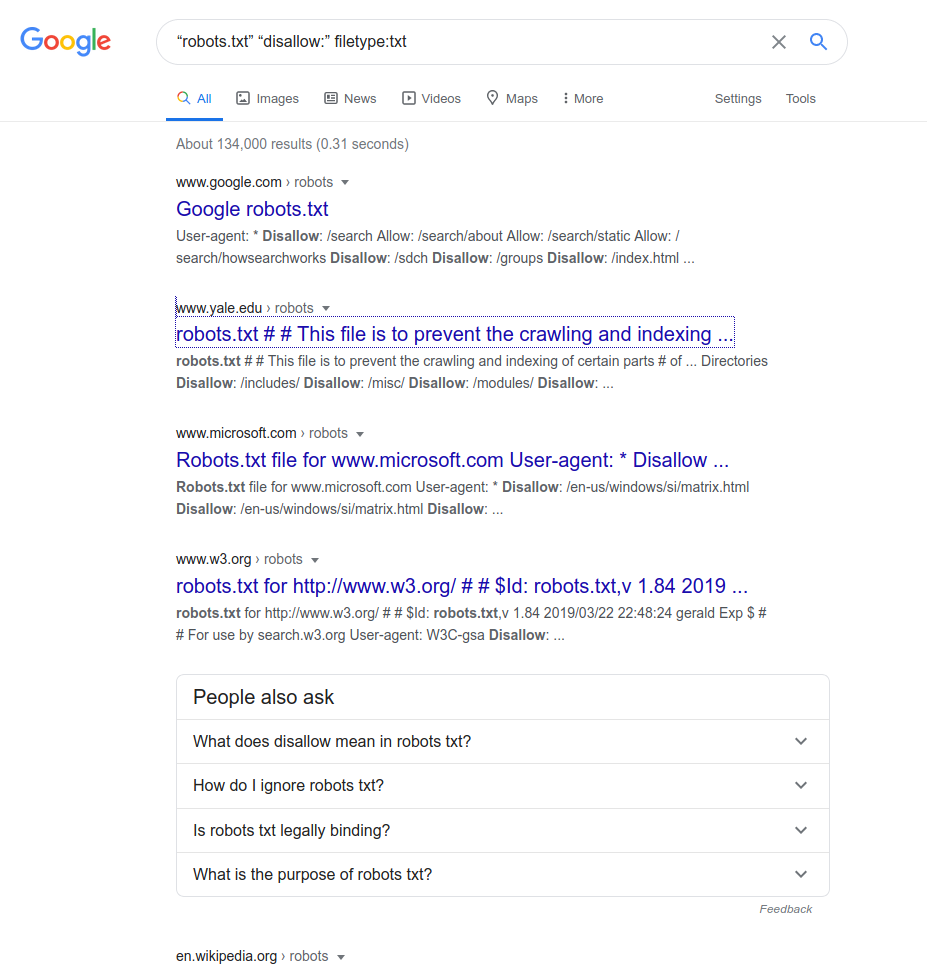
\includegraphics[width=.20\textwidth]{images/command12/base.png}\\
	
\includegraphics[width=.20\textwidth]{images/command12/result1.png}\\
	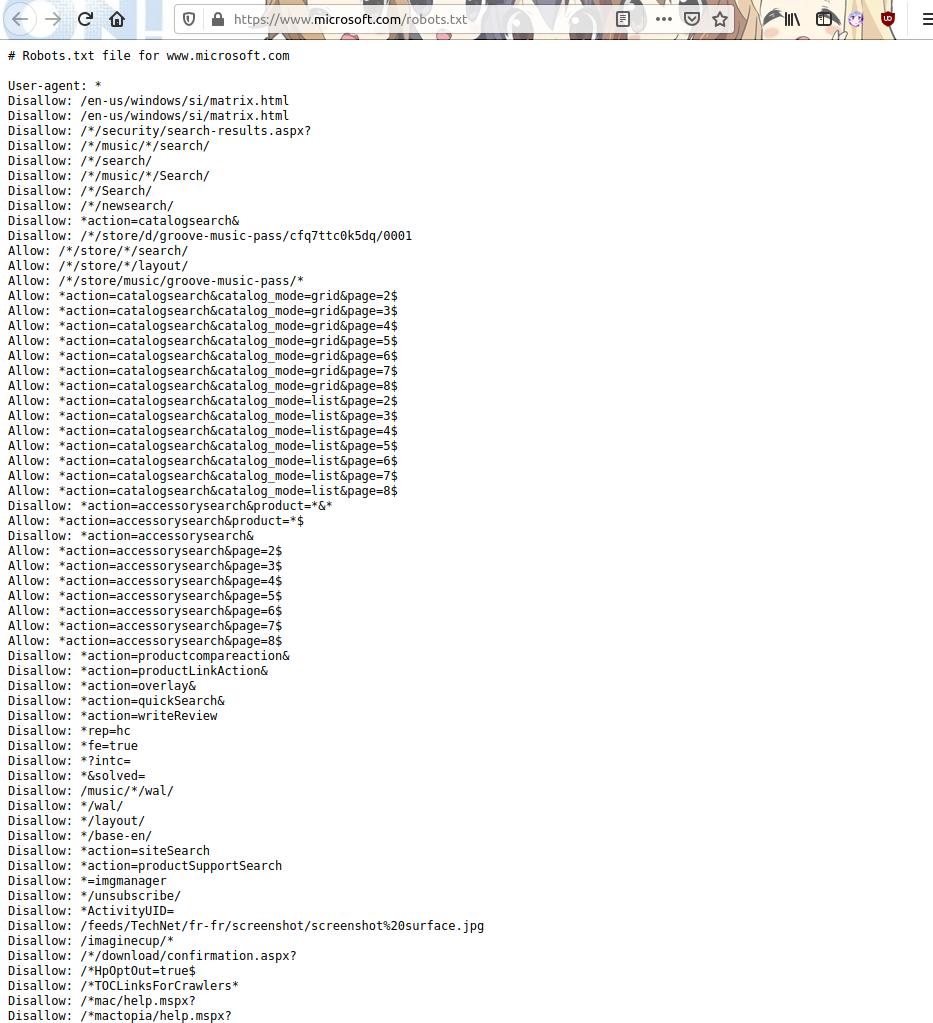
\includegraphics[width=.20\textwidth]{images/command12/result2.png}\\
	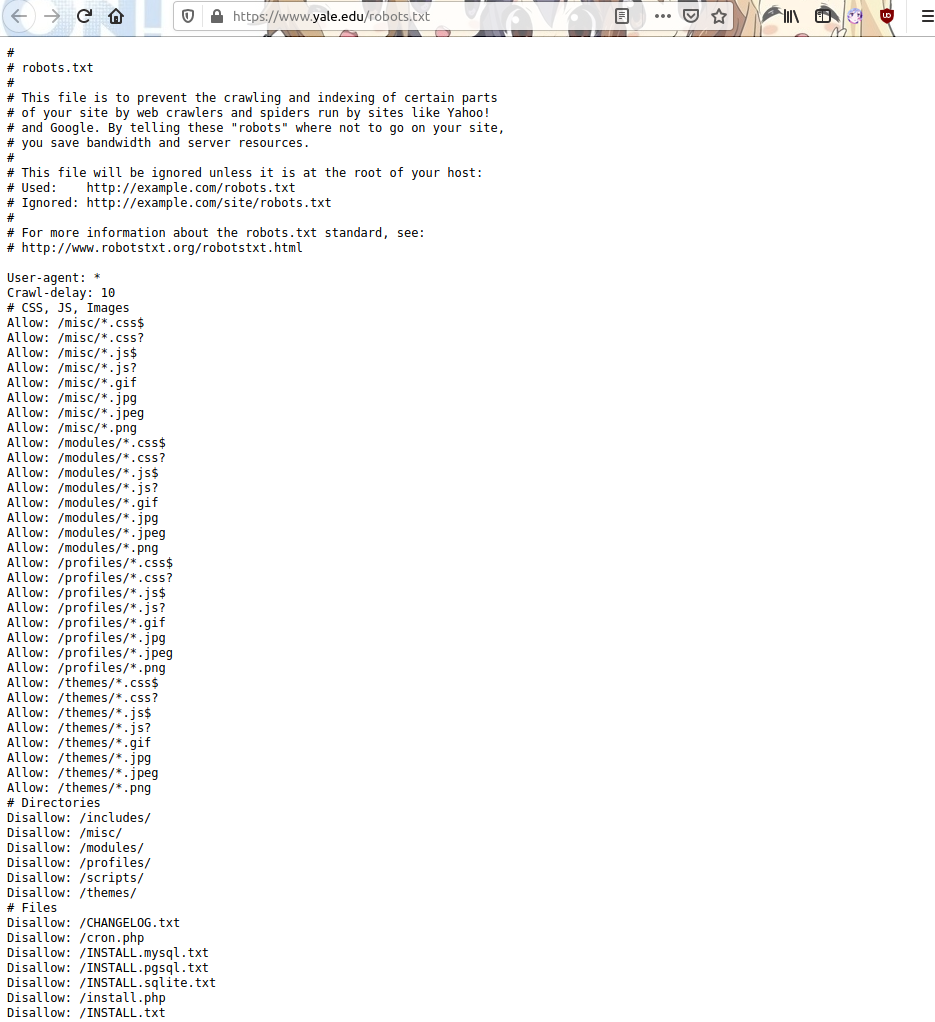
\includegraphics[width=.20\textwidth]{images/command12/result3.png}\\
\end{multicols}
\caption{Archivos de texto que tengan match en su contenido con \textit{(robots.txt|disallow:)}. Sirve para encontrar sitios que tengan declarado contenido que no desea que sea indexado por un buscador. Ahora esto se respeta en la práctica solo por voluntad de quien lo implementa, además que sirve para ver contenido de interés y sus rutas que podrían no estar presentes en una búsqueda.}
\label{FIG:command12}
\end{figure}



\subsubsection{\texttt{allintitle:restricted filetype:doc site:gov}}
\begin{figure}[H]
	\centering
\begin{multicols}{4}
	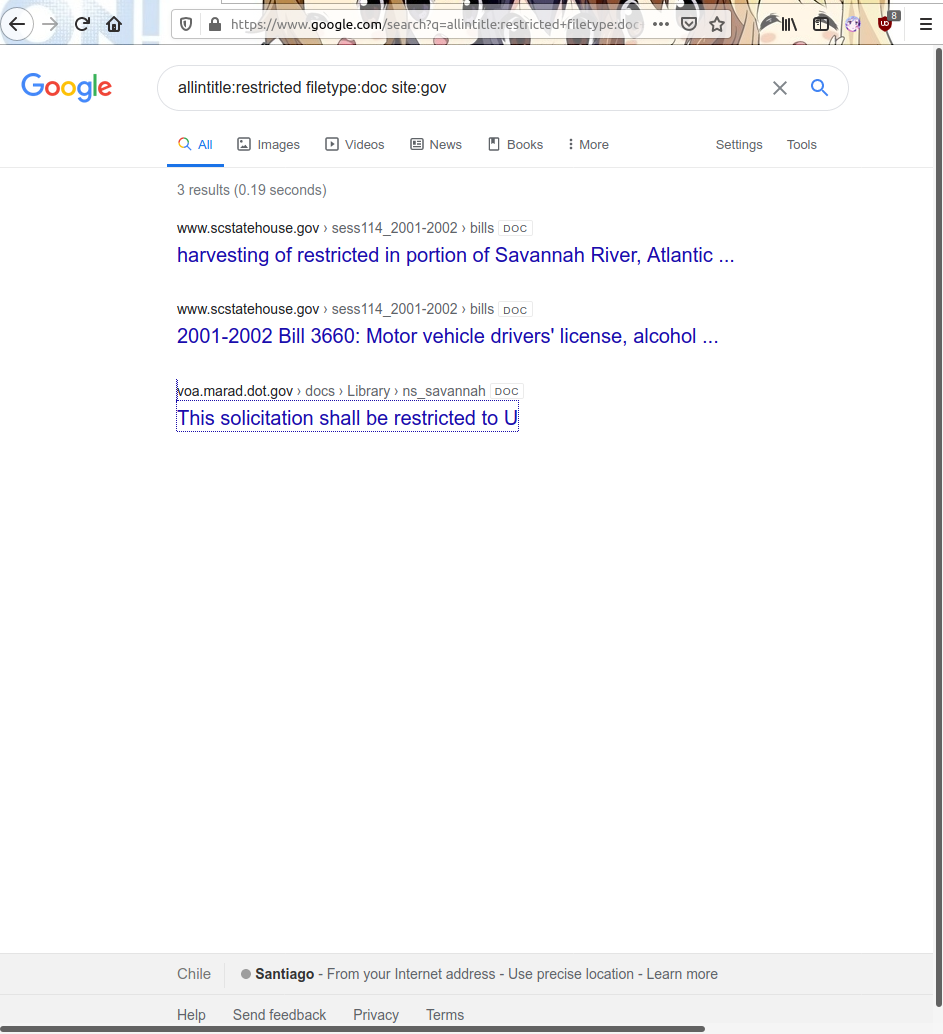
\includegraphics[width=.20\textwidth]{images/command13/base.png}\\
	
\includegraphics[width=.20\textwidth]{images/command13/result1.png}\\
	\includegraphics[width=.20\textwidth]{images/command13/result2.png}\\
	\includegraphics[width=.20\textwidth]{images/command13/result3.png}\\
\end{multicols}
\caption{Archivos .doc cuyo título contenga \textit{restricted} y que sean de un sitio del gobierno estadounidense. Lo que dice en el esquema, para nosotros poca utilizad tiene ya que este comando está regulado por google.}
\label{FIG:command13}
\end{figure}



\subsubsection{\texttt{index.of.dcim}}
\begin{figure}[H]
	\centering
\begin{multicols}{4}
	\includegraphics[width=.20\textwidth]{images/command14/base.png}\\
	\includegraphics[width=.20\textwidth]{images/command14/result1.png}\\
	\includegraphics[width=.20\textwidth]{images/command14/result2.png}\\
	\includegraphics[width=.20\textwidth]{images/command14/result3.png}\\
\end{multicols}
\caption{Entradas que contengan \textit{index.of.dcim}. Este esquema es típico de servidores expuestos o bien indexes de apache que no han sido cerrados y que contienen archivos de imagenes}
\label{FIG:command14}
\end{figure}

\section{En el informe de laboratorio deberá investigar a lo menos 2 comandos que no se encuentren en el listado de la actividad, entregando detalles de los resultados obtenidos y explicando cada uno de los componentes del comando.\cite{REF:google}\cite{REF:moz}}



\subsubsection{\texttt{filetype:log \enquote*{usuario} \enquote*{email}}}
\begin{figure}[H]
	\centering
\begin{multicols}{4}
	\includegraphics[width=.20\textwidth]{images/command15/base.png}\\
	\includegraphics[width=.20\textwidth]{images/command15/result1.png}\\
	\includegraphics[width=.20\textwidth]{images/command15/result2.png}\\
	\includegraphics[width=.20\textwidth]{images/command15/result3.png}\\
\end{multicols}
\caption{Archivos .log que con match \textit{usuario|email} en su contenido. Muchos logs son almacenados bajo esa extensión, lo cual resulta últil cuando los desarrolladores filtran información innecesaria en estos o bien los dejan expuestos. No solo pueden fltrar información personal, también información respecto a la infraestructura}
\label{FIG:command15}
\end{figure}



\subsubsection{\texttt{filetype:pem certificate}}
\begin{figure}[H]
	\centering
\begin{multicols}{4}
	\includegraphics[width=.20\textwidth]{images/command16/base.png}\\
	\includegraphics[width=.20\textwidth]{images/command16/result1.png}\\
	\includegraphics[width=.20\textwidth]{images/command16/result2.png}\\
	\includegraphics[width=.20\textwidth]{images/command16/result3.png}\\
\end{multicols}
\caption{Archivos .pem que con el texto certificate. Usado para encontrar certificados los cuales podrían contener desde solo llaves públicas hasta definiciones completas, útil en caso de necesitar forzar el acceso a un servidor ssh o realizar spoofing.}
\label{FIG:command16}
\end{figure}

\begin{thebibliography}{9}
	\bibitem{REF:moz}
	Moz - The Ultimate Guide to the Google Search Parameters.
	\textit{WebSite}.
	the-ultimate-guide-to-the-google-search-parameters.


	\bibitem{REF:google}
	Refine web searches
	\textit{Google Search Help}.
	https://support.google.com/websearch/answer/2466433?hl=en.

\end{thebibliography}

\end{document}